\documentclass[12pt,a4paper,oneside]{article}

\usepackage[left=3.5cm,top=3cm,right=2.5cm,bottom=3.5cm]{geometry}

\usepackage[english,italian]{babel}

\usepackage{lmodern}

\usepackage[utf8]{inputenc}

\usepackage[T1]{fontenc}

\usepackage{setspace}
\setstretch{1.35}

\usepackage{mathtools}

\usepackage[overload]{empheq}

\usepackage{amssymb}

\usepackage[bottom]{footmisc}

\usepackage[hidelinks]{hyperref}
\hypersetup{linktoc=all}

\usepackage{footnotebackref}

\usepackage{tablefootnote}

\usepackage[english,italian,nameinlink]{cleveref}
\crefname{algocf}{algoritmo}{algoritmi}
\crefname{section}{capitolo}{capitoli}

\usepackage{graphicx}

\usepackage{tikz}
\usetikzlibrary{shapes,arrows,positioning}
\usepackage{pgfplots}
\pgfplotsset{compat=newest}

\usepackage{multirow}

\usepackage{array}

\usepackage{longtable}

\usepackage{calc}

\usepackage[hypcap=true,labelformat=simple]{subcaption}
\renewcommand\thesubfigure{(\alph{subfigure})}

\usepackage[algoruled,longend,nofillcomment]{algorithm2e}
\SetAlgorithmName{Algoritmo}{algoritmo}{Elenco degli algoritmi}

\usepackage{fancyhdr}
\pagestyle{fancy}
\fancyhf{}
\renewcommand{\headrulewidth}{0pt}
\fancyfoot[R]{\thepage}

\usepackage[nopostdot,nonumberlist]{glossaries}
\makeglossaries

\bibliographystyle{IEEEtran}

\author{Georgiu Gabriel Claudiu}
\title{Adattamento e ottimizzazione di un algoritmo di superpixel per sequenze video}

\newacronym{SLIC}{SLIC}{Simple Linear Iterative Clustering}
\newacronym{OpenCV}{OpenCV}{Open Source Computer Vision Library}
\newacronym{Intel_TBB}{Intel TBB}{Intel Threading Building Blocks}
\newacronym{IDE}{IDE}{Integrated Development Environment}
\newacronym{API}{API}{Application Programming Interface}

\begin{document}



\selectlanguage{italian}
\pagenumbering{Roman}
\thispagestyle{empty}
\begin{spacing}{1.3}
	\begin{center}
		\noindent\makebox[\textwidth][c]{\Large\bf UNIVERSITÀ DEGLI STUDI DI GENOVA}
		\noindent\makebox[\textwidth][c]{\large\bf Facoltà di Ingegneria}	
		
		\begin{figure}[!htb]
			\centering
			
\includegraphics[height=30mm]{resources/logo.png}
		\end{figure}
	
		\begin{minipage}[!htb]{\textwidth}
			\begin{singlespace}
				\begin{center}
					{\itshape Corso di Laurea Triennale in\\ Ingegneria Elettronica e Tecnologie dell'Informazione} 
				\end{center}
			\end{singlespace}
		\end{minipage}
		
		\noindent\hrulefill\\
		
		\vfill
		
		\noindent\makebox[\textwidth][c]{
		\begin{minipage}[!htb]{.9\textwidth}
			\begin{center}
				{\LARGE\scshape Adattamento e ottimizzazione di un algoritmo di superpixel per sequenze video} 
			\end{center}
		\end{minipage}}
	\end{center}
	
	\vfill
	
	\noindent\begin{minipage}[t]{\textwidth-5.9cm}
		\textit{Relatore:}
		\begin{singlespace}
			\textbf{Prof. Lucio MARCENARO}\\
		\end{singlespace}
		\textit{Correlatore:}\\
		\textbf{Dott. Pietro MORERIO} 
	\end{minipage}%
	\noindent\begin{minipage}[t]{5.8cm}
		\textit{Candidato:}		
		\begin{singlespace}
			\textbf{Gabriel Claudiu GEORGIU}\\
			Matricola n. 3618343
		\end{singlespace}
	\end{minipage}%
	
	\vspace{2cm}
	
	\begin{center}
		\noindent\hrulefill\\
		\noindent\makebox[\textwidth][c]{Anno Accademico $2013  -  2014$}
	\end{center}	
\end{spacing}
\newpage



\selectlanguage{english}
\begin{center}
	\textbf{\Large Adaptation and optimization of a superpixel algorithm for video sequences}
\end{center}
\bigskip \bigskip
\begin{abstract}
\noindent The purpose of this thesis is to develop a \mbox{C++} program for the segmentation of video sequences into superpixels, in order to simplify and/or speed up later elaborations. The software has to be fast and efficient, so being able to balance superpixel accuracy and system performance is one of the biggest challenges. The first step of this work consists in optimizing the \mbox{C++} implementation of an existing image segmentation algorithm, while the second part focuses on how to adapt this algorithm to video records. The development and testing environment used during this thesis is Visual Studio 2012 running on a Windows~7 virtual machine, along with three external libraries: \acrshort{OpenCV} (for video and image elaborations), \acrshort{Intel_TBB} (for multi-threading operations) and Boost (for generating Gaussian noise). 
\end{abstract}
\newpage



\selectlanguage{italian}
\begin{spacing}{1.6}
\glossarystyle{altlist}
\printglossary[type=\acronymtype,title={Simboli e abbreviazioni}]
\end{spacing}
\newpage


\nocite{GEORGIU}
\tableofcontents
\newpage

\listoffigures
\listofalgorithms
\newpage



\listoftables
\newpage



\pagenumbering{arabic}
\section{Introduzione}\label{Introduzione}


La crescente diffusione di ``tecnologie indossabili'', ovvero di dispositivi e accessori dotati di componenti elettronici (come ad esempio occhiali e orologi \textit{smart}), richiede lo sviluppo di soluzioni software su misura che tengano conto della limitata capacità di calcolo e soprattutto della limitata autonomia energetica di tali dispositivi. In particolare, per quanto riguarda la categoria di apparecchi in grado di registrare filmati, è necessario un grande sforzo di ottimizzazione per garantire prestazioni perlomeno vicine al tempo reale quando si tratta di elaborazioni video.

In questa tesi si valuta la possibilità di adattare e ottimizzare per le sequenze video un algoritmo \cite{ACHANTA_SLIC} già affermato nel campo delle immagini per qualità e velocità di esecuzione. Tale algoritmo è denominato \acrshort{SLIC}~\cite{ACHANTA_SLIC} e consente di suddividere un'immagine in superpixel, ovvero in gruppi di pixel aventi proprietà simili. I superpixel costituiscono dunque una rappresentazione compatta dell'immagine, riducendone la complessità ed eliminando la ridondanza dei singoli pixel, e possono essere impiegati in svariate applicazioni, come ad esempio il riconoscimento di oggetti \cite{OBJECT_LOCALIZATION} oppure il \textit{tracking} \cite{TRACKING}. Rispetto alla moltitudine di algoritmi simili (fra cui \cite{GENERATIVE_PIETRO,COMANICIU_MEAN_SHIFT,MALIK_NORMALIZED_CUTS,FELZENSZWALB_GRAPH,GRID_SEAMS}), in questo elaborato viene scelto e approfondito \acrshort{SLIC}~\cite{ACHANTA_SLIC} per la sua relativa semplicità e velocità computazionale. Dato che un confronto dettagliato dei principali metodi per la generazione di superpixel esula dagli scopi di questo lavoro di laurea, per una comparazione esaustiva si rimanda a \cite{ACHANTA_SLIC}.

Sebbene la letteratura scientifica che tratta di superpixel sia molto vasta, finora si è focalizzata maggiormente sull'elaborazione di singole immagini e non di filmati. In ambito video i contributi finora più significativi sono \cite{DRUCKER_FAST_SUPERPIXELS_VIDEO,CHANG_TEMPORAL_SUPERPIXELS}. Tuttavia in \cite{DRUCKER_FAST_SUPERPIXELS_VIDEO} l'accuratezza dei superpixel è messa in secondo piano per ottenere ottime prestazioni, mentre \cite{CHANG_TEMPORAL_SUPERPIXELS} si basa su un approccio probabilistico che, seppur molto efficace, comporta tempi di esecuzione elevati. In \cite{SERRA_HAND_RECOGNITION} e \cite{VIDEOTRACE} la segmentazione in superpixel viene impiegata rispettivamente per il riconoscimento delle mani nei filmati girati in prima persona e per estrarre rappresentazioni tridimensionali degli oggetti presenti nei filmati, però in nessuno dei due casi viene approfondito in che modo i superpixel sono ottenuti a partire dai video.

Il carattere di quest'opera non è dunque completamente innovativo, dato che anche altri autori si sono occupati di superpixel applicati alle sequenze video, tuttavia l'apporto originale di questa tesi consiste nella trattazione dettagliata di come adattare e ottimizzare per i filmati un algoritmo rivelatosi molto efficace ed efficiente per singole immagini \cite{ACHANTA_SLIC}, con l'obiettivo di mantenere il più alta possibile la qualità dei superpixel ma riducendo al minimo i tempi di esecuzione. I progetti che ricorrono alla suddivisione in superpixel come passaggio intermedio, grazie a questo contributo, potrebbero trarre vantaggi in termini di prestazioni.

Il metodo presentato nella tesi si basa sul presupposto che esista una qualche correlazione tra frame consecutivi di una sequenza video, e sfruttando tale legame è possibile abbassare i tempi necessari all'elaborazione di \acrshort{SLIC}~\cite{ACHANTA_SLIC}. Per bilanciare la velocità di esecuzione con l'accuratezza della suddivisione in superpixel sono necessarie tuttavia ulteriori modifiche all'algoritmo, ispirate rispettivamente al filtraggio bayesiano e alla codifica video.

Il programma proposto è implementato in linguaggio \mbox{C++} e si basa su \textit{SLIC-Superpixels} (\url{http://github.com/PSMM/SLIC-Superpixels}), un progetto disponibile online. Gli strumenti utilizzati sono l'ambiente di sviluppo Microsoft Visual Studio insieme alle ultime versioni di alcune librerie esterne gratuite e \textit{open source}: per l'acquisizione e la gestione dei video e dei frame si impiega \gls{OpenCV}, mentre per incrementare le prestazioni del programma si ricorre a \gls{Intel_TBB}, che permette di sfruttare l'architettura \textit{multi-core} dei processori, rendendo quindi possibile l'esecuzione parallela di alcune parti dell'algoritmo implementato. Le librerie Boost vengono infine utilizzate per la generazione di rumore gaussiano.

A seguito di questo lavoro di laurea è stato scritto, e successivamente pubblicato sulla rivista \textit{IEEE Signal Processing Letters}, l'articolo ``Optimizing Superpixel Clustering for Real-Time
Egocentric-Vision Applications'' \cite{GEORGIU}.

\subsection{Organizzazione della tesi}
La tesi è organizzata secondo l'ordine cronologico di svolgimento: si inizia con una presentazione complessiva del lavoro che si intende compiere, si prosegue illustrando le metodologie e gli strumenti impiegati e si conclude infine con l'analisi e il commento dei risultati ottenuti, indicandone eventuali sviluppi futuri.

Il \hyperref[Introduzione]{primo capitolo} introduttivo offre una panoramica generale sugli argomenti trattati in questa tesi ed espone gli obiettivi prefissati.

Il \hyperref[Stato_arte]{secondo capitolo} presenta il contesto di svolgimento dell'elaborato di laurea: chiarisce il significato di superpixel, illustrando alcuni tipi di algoritmi per la loro generazione (si analizza in particolare \acrshort{SLIC}), e mostra i risultati più importanti ottenuti finora dalla comunità scientifica in questo ambito.

Nel \hyperref[Implementazione]{terzo capitolo} vengono descritte tutte le ottimizzazioni e le modifiche necessarie per adattare all'elaborazione di filmati l'algoritmo \acrshort{SLIC}, inizialmente progettato per le singole immagini.

Il \hyperref[Risultati]{quarto capitolo} riporta i risultati ottenuti dall'implementazione di \acrshort{SLIC} in linguaggio \mbox{C++}, sia quantitativamente sia qualitativamente. In particolare, sono presenti tabelle con dati relativi alle prestazioni e immagini (tratte dai filmati elaborati) che mostrano i punti di forza e gli svantaggi del metodo proposto.

Nel \hyperref[Conclusioni]{capitolo conclusivo} vengono fatte alcune considerazioni sui risultati ricavati durante lo svolgimento della tesi, illustrando infine alcuni possibili sviluppi futuri che prendano spunto da questo lavoro di laurea.
\newpage



\section{Stato dell'arte}\label{Stato_arte}


\subsection{Cosa sono i superpixel?}
Prima di procedere con la trattazione dettagliata del lavoro svolto in questa tesi, è utile soffermarsi per chiarire quale sia il significato del concetto di superpixel. Questo termine è stato introdotto per la prima volta da X. Ren e J. Malik in \cite{SUPERPIXEL} ($2003$) per descrivere gruppi di pixel aventi proprietà simili. Le immagini digitali possono essere descritte come una griglia di punti adiacenti, ciascuno dei quali avente una posizione e un colore ben definiti. I superpixel sono dunque insiemi contigui di punti con caratteristiche simili, che consentono di suddividere un'immagine complessa in macro-aree più agevoli da elaborare rispetto ai singoli pixel, fornendo quindi una rappresentazione di alto livello e alterando il meno possibile le caratteristiche dell'immagine originale. Le motivazioni che hanno portato gli autori di \cite{SUPERPIXEL} a introdurre i superpixel sono principalmente due: i pixel non sono entità naturali, ma il risultato della rappresentazione discreta delle immagini, e l'alto numero di pixel (anche per risoluzioni non troppo elevate) rende difficile la creazione di algoritmi efficienti.
\begin{figure}[!htb]	
	\centering
	\begin{subfigure}[t]{.325\textwidth}
		\phantomcaption
		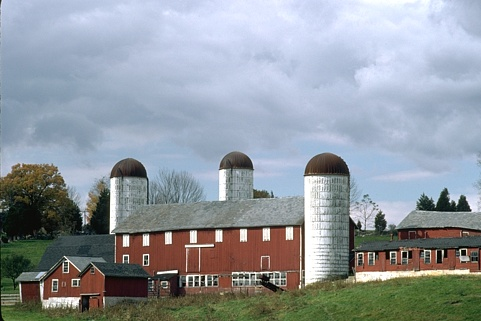
\includegraphics[width=\textwidth]{resources/images/es1_superpixel_originale.png}	
	\end{subfigure}%
	\hfill
	\begin{subfigure}[t]{.325\textwidth}
		\phantomcaption
		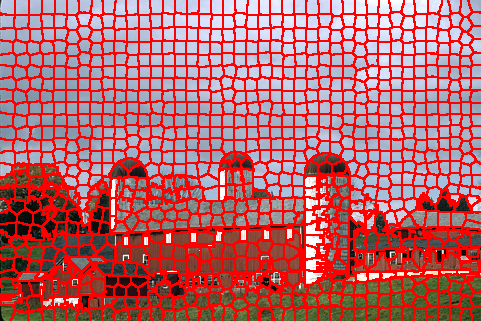
\includegraphics[width=\textwidth]{resources/images/es1_superpixel_contorni.png}
	\end{subfigure}%
	\hfill
	\begin{subfigure}[t]{.325\textwidth}
		\phantomcaption\label{es_superpixel_superpixel}
		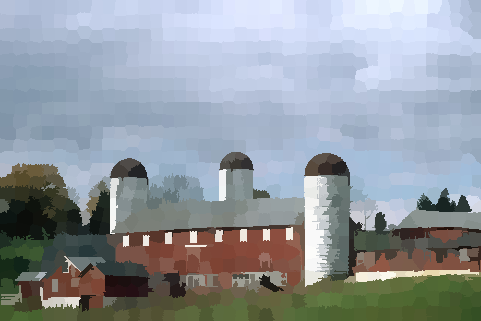
\includegraphics[width=\textwidth]{resources/images/es1_superpixel_superpixel.png}
	\end{subfigure}%
	\vspace{.01\textwidth}
	\begin{subfigure}[t]{.325\textwidth}
		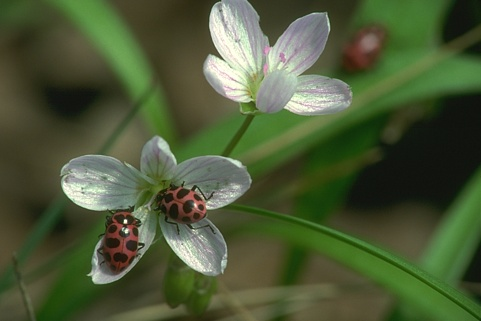
\includegraphics[width=\textwidth]{resources/images/es2_superpixel_originale.png}	
	\end{subfigure}%
	\hfill
	\begin{subfigure}[t]{.325\textwidth}
		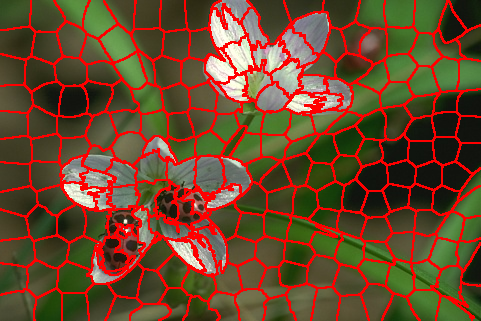
\includegraphics[width=\textwidth]{resources/images/es2_superpixel_contorni.png}
	\end{subfigure}%
	\hfill
	\begin{subfigure}[t]{.325\textwidth}
		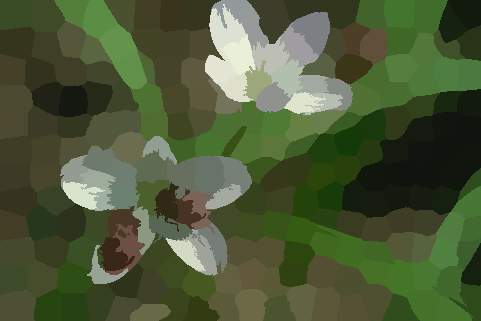
\includegraphics[width=\textwidth]{resources/images/es2_superpixel_superpixel.png}
	\end{subfigure}%
	\vspace{.01\textwidth}\setcounter{subfigure}{0}
	\begin{subfigure}[t]{.325\textwidth}
		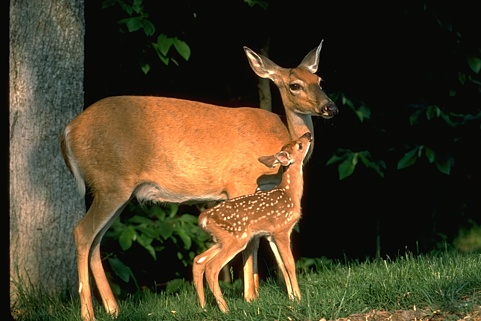
\includegraphics[width=\textwidth]{resources/images/es3_superpixel_originale.png}
		\caption{Immagine originale}	
	\end{subfigure}%
	\hfill
	\begin{subfigure}[t]{.325\textwidth}
		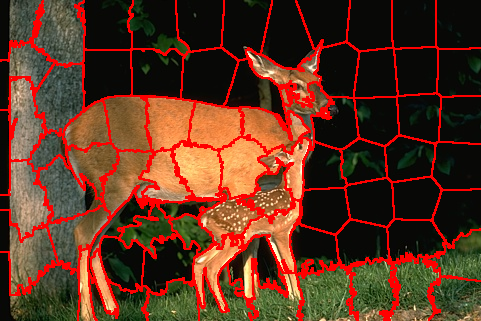
\includegraphics[width=\textwidth]{resources/images/es3_superpixel_contorni.png}
		\captionsetup{justification=centering}
		\caption{Contorni dei superpixel}
	\end{subfigure}%
	\hfill
	\begin{subfigure}[t]{.325\textwidth}
		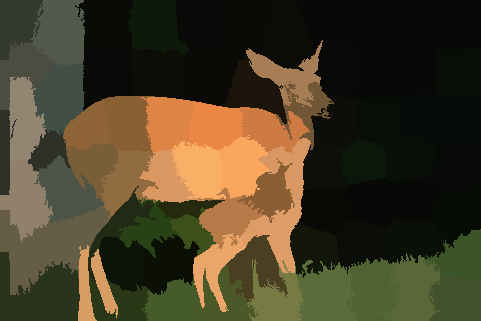
\includegraphics[width=\textwidth]{resources/images/es3_superpixel_superpixel.png}
		\caption{Immagine finale}
	\end{subfigure}%
	\caption{Esempio di immagini suddivise in superpixel}\label{es_superpixel}
\end{figure}
\\Nella \cref{es_superpixel} vengono proposti alcuni esempi di suddivisione in superpixel di figure appartenenti al \textit{Berkeley Segmentation Dataset}~\cite{BERKELEY_DATASET} (nella \cref{es_superpixel_superpixel} per ottenere il colore di ogni superpixel si calcola la media dei colori di tutti i singoli pixel contenuti al suo interno). Dato che un superpixel è per definizione un insieme di pixel aventi proprietà simili, nel seguito di questo elaborato il termine \textit{cluster} verrà spesso utilizzato come suo sinonimo.


\subsection{Algoritmi esistenti}
Al giorno d'oggi esistono numerosi metodi che consentono la suddivisione di immagini in superpixel (ad esempio \cite{ACHANTA_SLIC,GENERATIVE_PIETRO,COMANICIU_MEAN_SHIFT,MALIK_NORMALIZED_CUTS,FELZENSZWALB_GRAPH,GRID_SEAMS}) e le differenze principali consistono nelle forme, nelle caratteristiche e nelle dimensioni dei \textit{cluster} che vengono generati. Anche se la scelta del metodo più adatto dipende principalmente dall'ambito applicativo, i superpixel risultanti dovrebbero comunque rispettare i seguenti requisiti definiti in \cite{ACHANTA_SLIC}:
\begin{itemize}
	\item aderenza ai contorni degli oggetti presenti nelle immagini;
	\item facilità e velocità di calcolo;
\end{itemize}
In \cite{ACHANTA_SLIC} vengono inoltre individuate due categorie principali in cui è possibile classificare gli algoritmi per la generazione di superpixel:
\begin{itemize}
	\item\textbf{algoritmi basati su grafi}: ogni pixel rappresenta un nodo di un grafo, mentre i lati che collegano più nodi fra loro delineano il grado di similarità che intercorre fra i pixel connessi: i superpixel sono individuati minimizzando una certa funzione di costo definita nel grafo (\textit{Normalized Cuts}~\cite{MALIK_NORMALIZED_CUTS} è un esempio di algoritmo appartenente a questa tipologia);
	\item\textbf{algoritmi basati su variazioni del gradiente}: i pixel vengono suddivisi in gruppi o \textit{cluster} in modo ricorsivo, fino a quando non si verifica un determinato criterio di convergenza (\textit{\acrshort{SLIC}}~\cite{ACHANTA_SLIC}, l'algoritmo approfondito in questa tesi, funziona su questo principio).
\end{itemize}

\noindent\textbf{\Gls{SLIC}} è un algoritmo presentato in \cite{ACHANTA_SLIC} come metodo iterativo per la generazione di superpixel, avente i suoi punti di forza in velocità di esecuzione, efficienza nella gestione della memoria e aderenza ai contorni delle immagini. È ispirato all'algoritmo \textit{k-means clustering}, un procedimento che permette di suddividere un insieme di oggetti in $k$ gruppi in funzione delle loro caratteristiche. A differenza di \textit{k-means}, \gls{SLIC} si basa sulla ricerca locale invece che su quella globale, e ciò garantisce prestazioni migliori perché il numero di calcoli da effettuare è minore.

L'algoritmo preso in esame è composto da tre parti principali. Nella prima fase viene inizializzata una griglia (visibile nella \cref{SLIC_grid}) di dimensioni uguali all'immagine da elaborare, contenente punti che rappresentano i centri dei superpixel e che distano fra loro $S$, dove $S$ indica il passo di campionamento ed è una quantità che dipende dal numero totale di pixel della figura e dal numero di superpixel desiderato. Il secondo passaggio consiste nell'assegnare ogni pixel al \textit{cluster} adiacente, in una regione $2S \times 2S$, più vicino in termini di spazio e di colore, minimizzando la funzione distanza $D$ che definisce il grado di similarità fra due punti dell'immagine. La ricerca in un'area ristretta fa in modo che la dimensione attesa per ogni \textit{cluster} sia di circa $S \times S$ (come mostra la \cref{SLIC_grid}). Nell'ultima fase si aggiorna la posizione dei centri dei superpixel facendo la media delle posizioni dei singoli pixel contenuti al loro interno. Il secondo e il terzo passaggio sono ripetuti per un numero prefissato di volte, o fino a quando l'errore residuo $E$ non rientra in una certa soglia, $E$ rappresentando la variazione media della posizione dei centri dei \textit{cluster} fra due iterazioni consecutive.
\begin{figure}[!htb]
\centering
\begin{tikzpicture}[x=.1\textwidth,y=-.1\textwidth,scale=1.1]
	\draw[step=.1\textwidth,gray,very thin,line cap=rect] (0,0) grid (6,4);
	\draw[<->,ultra thick] (0,4) node (yaxis) [below] {$y$} |- (6,0) node (xaxis) [right] {$x$};
	\node[above left] at (-.1,-.1) {\small$0$};
	\node[above] at (1,-.1) {\small$S$};
	\node[left] at (-.1,1) {\small$S$~};
	\foreach \x in {2,...,5} \node[above] at (\x,-.1) {\small\x$S$};
	\foreach \y in {2,...,3} \node[left] at (-.1,\y) {\small\y$S$}; 
	\draw[very thick,line cap=rect,blue] (2,1) rectangle (4,3);
	\draw[dashed,thick,line cap=rect,red] (2.5,1.5) rectangle (3.5,2.5);
	\draw[->,thick] (3,2) -- (2.5,1.2);
	\draw[->,thick] (3,2) -- (3.8,1.5);
	\draw[->,thick] (3,2) -- (2.8,2.4);
	\node[below right,red] at (3,2.5) {\small $S \times S$};
	\node[below left,blue] at (4,3) {\small $2S \times 2S$};
\end{tikzpicture}
\caption{Area di ricerca locale $2S \times 2S$ dell'algoritmo \acrshort{SLIC}}\label{SLIC_grid}
\end{figure}
\\Anche se inizialmente è stato concepito per le immagini, durante questo lavoro le funzionalità di \gls{SLIC} vengono estese anche alla segmentazione di sequenze video, e il procedimento dettagliato viene illustrato negli \cref{Alg_vers_inter,Alg_vers_final} del \cref{Implementazione}.


\subsection{Implementazioni esistenti}
I progetti che trattano la generazione di superpixel sono numerosi, soprattutto se si considera l'elaborazione di singole immagini (\cite{ACHANTA_SLIC,GENERATIVE_PIETRO,COMANICIU_MEAN_SHIFT,MALIK_NORMALIZED_CUTS,FELZENSZWALB_GRAPH,GRID_SEAMS} sono alcuni esempi); negli ultimi anni c'è un crescente interesse verso i possibili impieghi dei superpixel anche nelle sequenze video, come dimostrano \cite{DRUCKER_FAST_SUPERPIXELS_VIDEO, CHANG_TEMPORAL_SUPERPIXELS}. In particolare, oltre al codice sorgente \mbox{C++} rilasciato direttamente dagli autori di \gls{SLIC} \cite{ACHANTA_SLIC}, sono presenti altre implementazioni basate sullo stesso algoritmo:
\begin{enumerate}
	\item[1)]\textit{SLIC-Superpixels} (\url{http://github.com/PSMM/SLIC-Superpixels}): progetto consultabile online che realizza l'algoritmo proposto in \cite{ACHANTA_SLIC} nel linguaggio \mbox{C++}, con l'ausilio della libreria esterna \gls{OpenCV}. Costituisce il punto di partenza del codice sorgente sviluppato durante questa tesi; 
	\item[2)]\textit{jSLIC} \cite{BOROVEC_jSLIC}: implementazione dell'algoritmo in linguaggio Java, con alcuni miglioramenti per aumentarne le prestazioni;
	\item[3)]\textit{gSLIC} \cite{YUHENG_gSLIC}: realizzazione di \gls{SLIC} basata sull'impiego di una scheda grafica dedicata, mediante l'utilizzo del \textit{framework} NVIDIA CUDA. Consente di ottenere risultati in tempo reale, a patto di disporre dell'hardware aggiuntivo necessario.
\end{enumerate}
\newpage





\section{Implementazione}\label{Implementazione}


Per implementare l'algoritmo \gls{SLIC} viene utilizzato l'\textit{\gls{IDE}} Visual Studio 2012, strumento di sviluppo proprietario di Microsoft, rilasciato in versione completa e gratuita agli studenti, in esecuzione su una macchina virtuale con sistema operativo Windows~7. Come linguaggio di programmazione si è scelto il \mbox{C++}, insieme alle librerie esterne \gls{OpenCV}, \gls{Intel_TBB} e Boost, presentate brevemente di seguito.
\newline

\noindent\textbf{\gls{OpenCV} (versione 2.4.9 - \url{http://opencv.org/})} è una libreria \textit{open source} distribuita in forma gratuita per qualsiasi tipo di utilizzo, contenente un elevato numero di algoritmi ottimizzati per la visione artificiale e l'apprendimento automatico. Le funzioni e le strutture dati implementate al suo interno consentono di effettuare sia operazioni di base su immagini e video, come l'estrapolazione dei singoli frame da un filmato, sia elaborazioni molto più complesse, come il riconoscimento dei volti, la creazione di modelli tridimensionali di oggetti o il tracciamento dei movimenti degli occhi. \gls{OpenCV} è nativa del \mbox{C++}, ma dispone anche di interfacce verso altri linguaggi di programmazione, come ad esempio \mbox{Java}, \mbox{Python} e \mbox{MATLAB}.
\newline

\noindent\textbf{\gls{Intel_TBB} (versione 4.2 - \url{http://www.threadingbuildingblocks.org/})} è una libreria \textit{open source} di \textit{template} \mbox{C++}. È gratuita per utilizzi non commerciali e consente ai programmi di sfruttare l'architettura \textit{multi-core} dei processori moderni, senza che il programmatore deva preoccuparsi di gestire manualmente i singoli \textit{thread}. Di particolare interesse per questo elaborato sono i metodi che permettono l'esecuzione parallela dei cicli di iterazioni presenti nel codice: ad esempio, la funzione \texttt{parallel\_for} di questa libreria corrisponde al normale ciclo \texttt{for} del linguaggio \mbox{C++} standard, con la differenza che nel primo caso le istruzioni vengono eseguite, per quanto possibile, in parallelo. Un approccio di questo genere, che trae vantaggio dal \textit{multi-threading}, offre ottimi risultati e prestazioni quando i dati possono essere elaborati indipendentemente gli uni dagli altri, come spesso accade con i pixel in un'immagine digitale.
\newline

\noindent\textbf{Boost (versione 1.56.0 - \url{http://www.boost.org/})} è una collezione di librerie \textit{open source} gratuite, con una licenza molto permissiva anche per utilizzi in ambito commerciale. Le strutture dati e i metodi presenti al suo interno estendono le funzionalità offerte dal \mbox{C++} standard e trovano impiego in una vasta gamma di applicazioni, come ad esempio l'algebra lineare, le espressioni regolari e la creazione di numeri pseudocasuali. In questa tesi l'utilizzo delle librerie Boost è limitato alla generazione di rumore gaussiano.

\subsection{Superpixel da sequenze video}
Il lavoro svolto durante questo elaborato di laurea è basato su un'implementazione già esistente dell'algoritmo \gls{SLIC}: il progetto \textit{SLIC-Superpixels}, reperibile online all'indirizzo web \url{http://github.com/PSMM/SLIC-Superpixels}. Siccome il codice originale è concepito per processare solamente singole immagini, la prima operazione da fare è apportare alcune modifiche che consentano anche la gestione delle sequenze video. Per fare ciò, si può interpretare un filmato come una serie di immagini in rapida successione. Pertanto, per segmentare un video in superpixel, inizialmente si può pensare di elaborare ogni singolo frame indipendentemente dagli altri, come illustrato nell'\cref{Alg_vers_init} e più dettagliatamente nell'\cref{Alg_vers_inter}.
\begin{algorithm}[!htb]
	\caption{SLIC applicato a ogni frame}
	\label{Alg_vers_init}
	\SetKwData{frame}{frame}
	\SetKwData{video}{video}
	\SetKwFunction{eseguiSLICsuImmagine}{eseguiSLICsuImmagine}
	\SetKwInOut{Input}{Input}\SetKwInOut{Output}{Output}
	\BlankLine
	\Input{Video da segmentare in superpixel}
	\Output{Video suddiviso in superpixel}
	\BlankLine
	\ForEach{\frame in \video}
	{
	converti \frame a spazio colore \mbox{LAB}\;
	\BlankLine
	\tcc{con numero di iterazioni costante = 10}
	\eseguiSLICsuImmagine{\frame};
	\BlankLine
	riconverti \frame a spazio colore \mbox{RGB}\;
	salva \frame\;
	}
\end{algorithm}
\\\noindent Questo approccio funziona, ma ha due svantaggi:
\begin{enumerate}
	\item[a)]tra due frame consecutivi, anche molto simili fra loro, la forma e/o la posizione della maggior parte dei superpixel cambia in modo significativo, rendendoli quindi ``instabili'' per tutta la durata del video;
	\item[b)]le informazioni ottenute relative ai superpixel devono essere resettate ai valori di default dell'algoritmo a ogni nuovo frame, e tale operazione comporta un dispendio di risorse.
\end{enumerate}
\begin{algorithm}[!htb]
	\caption{SLIC applicato a ogni frame nel dettaglio}
	\label{Alg_vers_inter}
	\SetKwData{frame}{frame}
	\SetKwData{video}{video}
	\SetKwData{pixel}{pixel}
	\SetKwFunction{clusterDiAppartenenza}{clusterDiAppartenenza}
	\SetKwFunction{distanzaDaCluster}{distanzaDaCluster}
	\SetKwInOut{Input}{Input}\SetKwInOut{Output}{Output}
	\BlankLine
	\Input{Video da segmentare in superpixel}
	\Output{Video suddiviso in superpixel}
	\BlankLine
	\ForEach{\frame in \video}
	{
	converti \frame a spazio colore \mbox{LAB}\;
	\tcc{Inizializzazione}
	inizializza centri dei \textit{cluster} $C_k = \left[L_k,A_k,B_k,x_k,y_k\right]^T$ campionando i \pixel del \frame a passo costante $S$\;
	sposta centri dei \textit{cluster} nel punto a gradiente più basso in un intorno di $3 \times 3$ \pixel\;
	\ForEach{\pixel in \frame}
	{
	$\clusterDiAppartenenza{\pixel} = -1$\;
	$\distanzaDaCluster{\pixel} = \infty$\;
	}
	\For{$n = 1$ \KwSty{to} $10$}
	{
	\tcc{Assegnazione}
	\ForEach{centro di cluster $C_k$}
	{
	\ForEach{\pixel in un intorno $2S \times 2S$ di $C_k$}
	{
	calcola distanza $D$ fra \pixel e $C_k$\;
	\If{$D < \distanzaDaCluster{\pixel}$}
	{
	$\clusterDiAppartenenza{\pixel} = k$\;
	$\distanzaDaCluster{\pixel} = D$\;
	}
	}
	}
	\tcc{Aggiornamento}
	calcola i nuovi centri dei \textit{cluster}\;
	}
	riconverti \frame a spazio colore \mbox{RGB}\;
	salva \frame\;
	}
\end{algorithm}


\subsection{Ottimizzazione del codice}\label{Ottimizzazione_codice}
Prima di illustrare ulteriori modifiche all'algoritmo al fine di adattarlo meglio all'elaborazione dei video, di seguito vengono descritti qualitativamente tutti i cambiamenti e/o le aggiunte al codice sorgente originale di \textit{SLIC-Superpixels}, con lo scopo di rendere l'esecuzione del programma più veloce ed efficiente. I miglioramenti ottenuti dal punto di vista quantitativo sono mostrati nel \cref{Risultati}.

\subsubsection{Aggiornamento all'ultima versione di \acrshort{OpenCV}}
Nel progetto \textit{SLIC-Superpixels} vengono impiegate strutture dati tipiche delle prime versioni di \gls{OpenCV}, pertanto è bene installare un'edizione più recente della libreria, in modo da poter usufruire delle nuove \textit{\gls{API}} specifiche del linguaggio \mbox{C++}. I tipi di dato obsoleti attualmente utilizzati nel codice sorgente di \textit{SLIC-Superpixels}, come ad esempio \texttt{IplImage}, \texttt{cvPoint} e \texttt{cvScalar} vengono rispettivamente sostituiti da \texttt{Mat}, \texttt{Point} e \texttt{Vec3b}. Tale cambiamento comporta una riduzione non indifferente dei tempi di esecuzione del programma, come attesta la \cref{EDSH_videos_perf_new_OpenCV} del \cref{Risultati_opt}.

\subsubsection{Ottimizzazione per la memoria \textit{cache}}
La memoria \textit{cache} è una memoria temporanea di capienza relativamente ridotta (tipicamente da qualche centinaio di KB fino ad alcuni MB) che in compenso fornisce tempi di accesso molto più bassi rispetto alla tradizionale \mbox{RAM}, pertanto viene adoperata per salvare le istruzioni e/o i dati utilizzati più frequentemente. La \textit{cache} si basa su due principi fondamentali: la località spaziale, ovvero la probabilità che accedendo a un dato si deva accedere anche a quelli memorizzati in indirizzi vicini, e la località temporale, cioè la probabilità che un dato a cui si è fatto riferimento venga richiesto nuovamente in tempi brevi. Per poter sfruttare la località spaziale è necessario dunque che i valori delle matrici utilizzate nel programma vengano salvati in zone di memoria adiacenti, e ciò si può ottenere impiegando vettori monodimensionali. Nel caso di vettori bidimensionali è opportuno verificare se i dati vengono salvati per righe o per colonne e agire di conseguenza. Ad esempio, il tipo \texttt{Mat} della libreria \gls{OpenCV} memorizza gli elementi riga per riga\footnote{Fonte: \url{http://docs.opencv.org/modules/core/doc/basic_structures.html\#mat}}, quindi, per sfruttare la \textit{cache} e avere prestazioni massime, è meglio scandire gli oggetti di tipo \texttt{Mat} riga per riga. Si osserva infine che un vettore monodimensionale può essere trattato come se avesse due dimensioni (\cref{vector_relation}), pertanto, da un punto di vista prestazionale, quando possibile è conveniente ricorrere all'utilizzo di vettori monodimensionali al posto di matrici bidimensionali. Come si può dedurre dalla \cref{vector_relation}, la relazione che lega le due strutture di dati in esame è la seguente:
\\\texttt{vettore2D[y][x] = vettore1D[y $\cdot$ numeroDiColonne + x]}.
\begin{figure}[!htb]
\centering
\vspace{.2cm}
\begin{tikzpicture}[x=.1\textwidth,y=-.1\textwidth,scale=.8]
	\foreach \x in {0,...,2} \filldraw[very thick,line cap=rect,fill=brown,fill opacity=.5] (\x,0.0) rectangle (\x+1,1.0);
	\foreach \x in {0,...,2} \filldraw[very thick,line cap=rect,fill=red,fill opacity=.5] (\x,1.0) rectangle (\x+1,2.0);
	\foreach \x in {0,...,2} \filldraw[very thick,line cap=rect,fill=violet,fill opacity=.5] (\x,2.0) rectangle (\x+1,3.0);
	\foreach \x in {0,...,2} \filldraw[very thick,line cap=rect,fill=blue,fill opacity=.5] (\x,3.0) rectangle (\x+1,4.0);

	\foreach \y in {1,...,4} \foreach \x in {1,...,3} \node at (\x-.5\x,\y-.5\y) {$E_{\y\x}$};
	
	\foreach \x in {0,...,2} \filldraw[very thick,line cap=rect,fill=brown,fill opacity=.5] (\x+5,-0.75) rectangle (\x+6,0.25);
	\foreach \x in {0,...,2} \filldraw[very thick,line cap=rect,fill=red,fill opacity=.5] (\x+5,0.75) rectangle (\x+6,1.75);
	\foreach \x in {0,...,2} \filldraw[very thick,line cap=rect,fill=violet,fill opacity=.5] (\x+5,2.25) rectangle (\x+6,3.25);
	\foreach \x in {0,...,2} \filldraw[very thick,line cap=rect,fill=blue,fill opacity=.5] (\x+5,3.75) rectangle (\x+6,4.75);
	\foreach \x in {0,1.5,3} \draw[->,very thick] (8.0,-0.25+\x) -- (8.5,-0.25+\x) -- (8.5,0.5+\x) -- (4.5,0.5+\x) -- (4.5,1.25+\x) -- (5.0,1.25+\x);

	\foreach \y in {1,...,4} \foreach \x in {1,...,3} \node at (\x+5-.5\x,1.5*\y-1.75) {$E_{\y\x}$};
	
	\node[above right] at (0.0,0.0) {\texttt{vettore2D[4][3]}};
\end{tikzpicture}

\vspace{.5cm}

\begin{tikzpicture}[x=.1\textwidth,y=-.1\textwidth,scale=.8]
	\foreach \x in {0,...,2} \filldraw[very thick,line cap=rect,fill=brown,fill opacity=.5] (\x,0.0) rectangle (\x+1,1.0);
	\foreach \x in {3,...,5} \filldraw[very thick,line cap=rect,fill=red,fill opacity=.5] (\x,0.0) rectangle (\x+1,1.0);
	\foreach \x in {6,...,8} \filldraw[very thick,line cap=rect,fill=violet,fill opacity=.5] (\x,0.0) rectangle (\x+1,1.0);
	\foreach \x in {9,...,11} \filldraw[very thick,line cap=rect,fill=blue,fill opacity=.5] (\x,0.0) rectangle (\x+1,1.0);

	\foreach \y in {1,...,4} \foreach \x in {1,...,3} \node at (3.0*\y-3+\x-.5\x,0.5) {$E_{\y\x}$};
	
	\node[above right] at (0.0,0.0) {\texttt{vettore1D[12]}};
\end{tikzpicture}
\caption{Relazione tra vettori bidimensionali e vettori monodimensionali}\label{vector_relation}
\end{figure}

\subsubsection{Ottimizzazione del calcolo della distanza}
Gli autori di \cite{ACHANTA_SLIC} propongono la seguente formula per il calcolo della distanza fra due pixel di un'immagine:
\begin{equation}\label{sup_distance}
D = \sqrt{{d_c}^2 + \left(\frac{d_s}{S}\right)^2 \cdot m^2}
\end{equation}
dove $d_c$ e $d_s$ rappresentano rispettivamente la distanza nel colore e nello spazio, $S$ è il passo di campionamento dell'algoritmo mentre $m$ è un fattore peso regolabile che indica l'importanza di $d_s$ rispetto a $d_c$. Siccome il calcolo di $D$ è necessario solo per il confronto con altre distanze ricavate con la stessa formula, e il valore assoluto di $D$ non è richiesto, sapendo che:
\begin{equation*}
a \leq b \quad \Leftrightarrow \quad \sqrt{a} \leq \sqrt{b} \qquad \forall a,b \in \mathbb{R_+}
\end{equation*}
l'\cref{sup_distance} si può modificare e riscrivere come:
\begin{equation}\label{sup_distance_opt}
D = {d_c}^2 + \beta \cdot {d_s}^2 \qquad \text{dove} \qquad \beta = \left(\frac{m}{S}\right)^2
\end{equation}
Dal momento che il valore di $D$ viene calcolato molto spesso durante l'esecuzione del programma, conviene ricavare e salvare la variabile $\beta$ nella fase di inizializzazione. È inoltre opportuno evitare di usare funzioni di libreria per l'elevamento a potenza, dato che risulta più efficiente utilizzare direttamente la moltiplicazione del valore per se stesso.

L'ottimizzazione per la memoria \textit{cache}, congiunta alle modifiche al calcolo della distanza appena descritte, consente un notevole miglioramento delle prestazioni del programma, come testimonia la \cref{EDSH_videos_perf_cache_distance} del \cref{Risultati_opt}.

\subsubsection{Altre ottimizzazioni minori e \textit{refactoring}}
Le ottimizzazioni marginali apportate al codice sorgente sono descritte di seguito:
\begin{itemize}
	\item\textbf{passaggio per riferimento degli oggetti complessi}: in questo modo si evita di dover fare una copia dell'oggetto in memoria, operazione che può risultare onerosa per i dati di grandi dimensioni (come può essere il tipo \texttt{Mat} di \gls{OpenCV}). Per le variabili più semplici, come ad esempio quelle di tipo \texttt{int}, conviene invece il passaggio per valore;
	\item\textbf{calcolo e salvataggio iniziale delle variabili più usate}: se nel programma sono presenti molti calcoli richiamati spesso e che hanno in comune una parte costante, è opportuno calcolare e salvare tale costante nella fase di inizializzazione, come avviene ad esempio con il parametro $\beta$ (\cref{sup_distance_opt}), chiamato \texttt{distanceFactor} nel codice sorgente proposto;
	\item\textbf{evitare la chiamata a funzione quando c'è una soluzione più immediata}: le frequenti chiamate di funzioni rallentano l'esecuzione del programma, quindi, dove possibile, conviene ricorrere a soluzioni più semplici e dirette. Per esempio, quando si ha l'elevamento a potenza, risulta più veloce moltiplicare il valore per se stesso invece di chiamare una funzione come \texttt{pow};
	\item\textbf{utilizzo del preincremento invece del postincremento}: per gli oggetti e le variabili che dispongono degli operatori \texttt{++} e \texttt{-{}-} è preferibile usare la notazione \texttt{++var} al posto di \texttt{var++}, poiché il secondo caso comporta la creazione di una copia temporanea in memoria.
\end{itemize}

\noindent Il \textit{refactoring} consiste nell'alterare la struttura interna del codice sorgente senza cambiarne il comportamento esterno\footnote{Fonte: \url{http://refactoring.com/}}, ovvero nell'effettuare piccole modifiche che rendano il codice più facile da leggere, comprendere e modificare in futuro. Rispetto al progetto originale \textit{SLIC-Superpixels}, nel lavoro sviluppato in questa tesi si utilizzano nomi più descrittivi per i metodi e per le variabili, vengono aggiunti ulteriori commenti e vengono eliminate le ridondanze di alcune parti del codice. La \cref{EDSH_videos_perf_minor_refact} del \cref{Risultati_opt} quantifica il miglioramento di prestazioni ottenuto.

\subsubsection{\textit{Multi-threading}}
Tramite la libreria \gls{Intel_TBB} si può sfruttare l'architettura \textit{multi-core} dei processori moderni, che consente l'esecuzione contemporanea di alcune parti di codice grazie alla possibilità di avviare più \textit{thread} in parallelo (operazione chiamata \textit{multi-threading}). Nel progetto proposto viene impiegata solamente una delle funzioni messe a disposizione dalla libreria, ovvero la \texttt{parallel\_for}: si tratta di un metodo che va utilizzato al posto del ciclo \texttt{for} già implementato nel \mbox{C++}. Mentre con la classica istruzione \texttt{for} ogni iterazione viene eseguita sequenzialmente, dopo il completamento di quella che la precede, nel caso di \texttt{parallel\_for} vengono invece avviati più cicli contemporaneamente, pertanto, per un corretto funzionamento, è essenziale che ogni ciclo sia indipendente dagli altri. L'implementazione del \textit{multi-threading} consente al programma di dimezzare i tempi di esecuzione, come dimostra la \cref{EDSH_videos_perf_mthread} del \cref{Risultati_opt}.

\subsection{Modifiche all'algoritmo}\label{Modifiche_algoritmo}
Gli autori di \cite{ACHANTA_SLIC} sostengono che $10$ iterazioni dell'algoritmo \gls{SLIC} siano sufficienti per avere buoni risultati per la maggioranza delle immagini. In questa tesi, dal momento che si prendono in esame i video, si preferisce invece optare per la valutazione dell'errore residuo $E$ (calcolato sui centri dei superpixel): si imposta una soglia massima di errore ammissibile $E_{th}$ e si ripetono le istruzioni dell'algoritmo fino a quando tale errore non converge al valore di $E_{th}$ desiderato. Rispetto alla scelta di un numero fisso di iterazioni, questo metodo ha alcuni punti a favore:
\begin{enumerate}
	\item[a)]la precisione del risultato è sempre garantita, poiché dipende esclusivamente dal valore minimo di $E_{th}$ scelto. Se il numero di ripetizioni fosse fisso, non si potrebbe avere la certezza di ottenere lo stesso livello di precisione per tutti i frame;
	\item[b)]le risorse vengono impiegate in maniera più efficiente, evitando l'esecuzione di iterazioni superflue dopo il raggiungimento della soglia di errore.
\end{enumerate}

\noindent Finora si è ipotizzato che i frame di un video fossero indipendenti, ma un filmato può anche essere considerato come un flusso di immagini interconnesse fra loro, dove ognuna di esse dipende in qualche misura da quella che la precede. In questo modo è possibile formulare una soluzione migliore rispetto a quella proposta inizialmente: i superpixel di ogni frame, a esclusione del primo, invece che essere impostati a default (come in \cref{es_init_no_memory}), vengono inizializzati con i dati risultanti dall'analisi del frame precedente (elaborazione ``con memoria'', visibile nella \cref{es_init_memory}).
\begin{figure}[!htb]	
	\centering
	\begin{subfigure}[t]{.325\textwidth}
		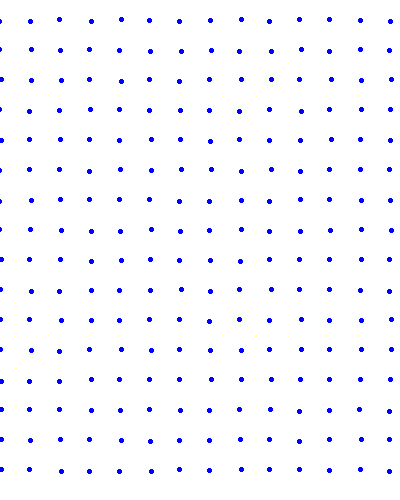
\includegraphics[width=\textwidth]{resources/images/mascheraIntermedia_no_memory.png}
		\captionsetup{justification=centering}
		\caption{Griglia di inizializzazione fissa di passo $S$}	
	\end{subfigure}%
	\hfill
	\begin{subfigure}[t]{.325\textwidth}
		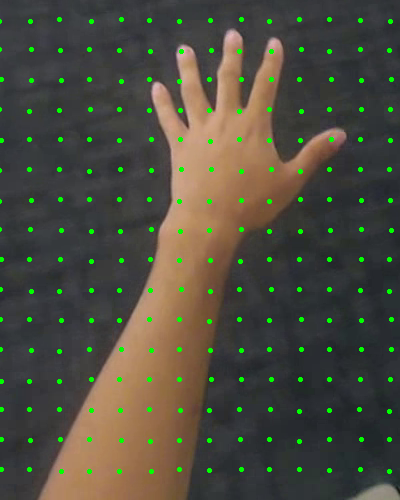
\includegraphics[width=\textwidth]{resources/images/inizializzazioneFrameAttuale_no_memory.png}
		\captionsetup{justification=centering}
		\caption{Inizializzazione del frame $k$ con la griglia di default}
	\end{subfigure}%
	\hfill
	\begin{subfigure}[t]{.325\textwidth}
		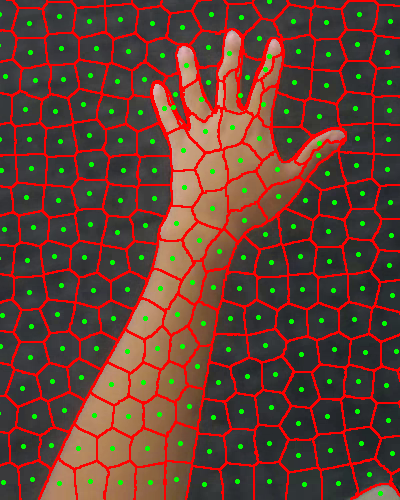
\includegraphics[width=\textwidth]{resources/images/risultatoFrameAttuale_no_memory.png}
		\captionsetup{justification=centering}
		\caption{Risultato del frame $k$}
	\end{subfigure}%
	\caption{Inizializzazione di default senza memoria}\label{es_init_no_memory}
\end{figure}
\\È importante osservare come nella \cref{es_init_no_memory} l'unica informazione necessaria per l'inizializzazione sia relativa alla posizione dei centri dei \textit{cluster} mentre nella \cref{es_init_memory}, oltre alla posizione dei centri, viene utilizzata anche la suddivisione in superpixel ricavata nel frame precedente. In particolare, nella \cref{es_init_memory_intermedio} si può notare come le differenze tra il frame $k$ e \mbox{$k - 1$} siano minime: i contorni della mano ricavati dal frame \mbox{$k - 1$} combaciano quasi perfettamente con quelli del frame $k$, pertanto il numero di iterazioni necessarie alla convergenza è minore rispetto al caso presentato in \cref{es_init_no_memory}.
\begin{figure}[!htb]	
	\centering
	\begin{subfigure}[t]{.325\textwidth}
		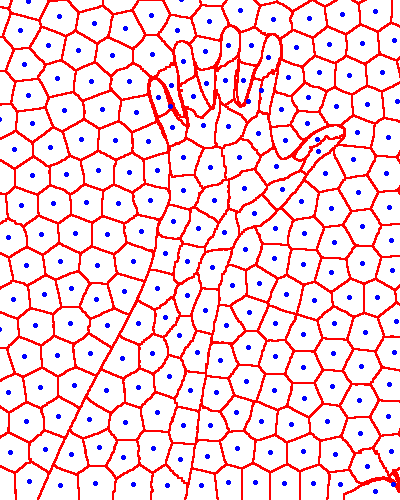
\includegraphics[width=\textwidth]{resources/images/mascheraIntermedia_memory.png}
		\captionsetup{justification=centering}
		\caption{Griglia risultante dall'elaborazione del frame \mbox{$k - 1$}}	
	\end{subfigure}%
	\hfill
	\begin{subfigure}[t]{.325\textwidth}
		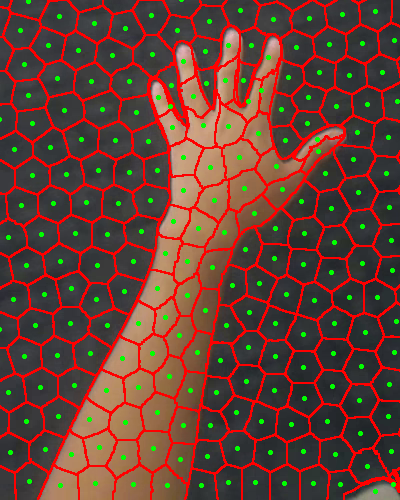
\includegraphics[width=\textwidth]{resources/images/inizializzazioneFrameAttuale_memory.png}
		\captionsetup{justification=centering}
		\caption{Inizializzazione del frame $k$ utilizzando la griglia del frame \mbox{$k - 1$}}\label{es_init_memory_intermedio}
	\end{subfigure}%
	\hfill
	\begin{subfigure}[t]{.325\textwidth}
		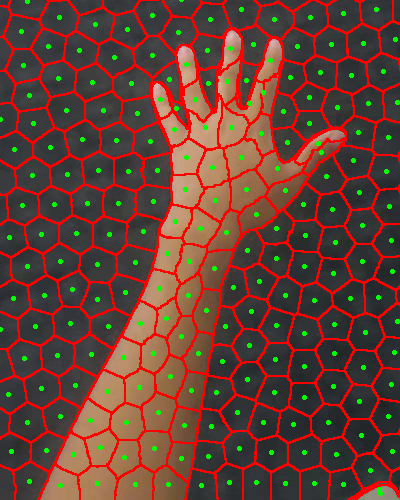
\includegraphics[width=\textwidth]{resources/images/risultatoFrameAttuale_memory.png}
		\captionsetup{justification=centering}
		\caption{Risultato del frame $k$}
	\end{subfigure}%
	\caption{Inizializzazione con memoria}\label{es_init_memory}
\end{figure}
\\L'algoritmo risulta dunque più efficiente, ci sono meno sprechi di risorse e i superpixel variano meno la loro forma e posizione tra un frame e il successivo. Inoltre la quantità di calcoli da eseguire cambia a seconda delle caratteristiche del filmato: se una sequenza video varia poco, i fotogrammi sono molto simili fra loro, quindi l'algoritmo converge più velocemente; se invece una sequenza è dinamica, i frame si assomigliano di meno, perciò sono necessari più calcoli e più tempo per la convergenza. Questo approccio, che sfrutta la ``memoria'' del filmato, si rivela molto efficiente per quanto riguarda i tempi di esecuzione, però ha lo svantaggio di introdurre un effetto indesiderato che si manifesta in modo proporzionale alla quantità di frame elaborati. Tale effetto, descritto più dettagliatamente nel \cref{Drifting_effect}, in questo elaborato viene chiamato effetto \textit{drifting} e consiste nella comparsa di superpixel non aderenti ai contorni degli oggetti presenti nell'immagine, che assumono spesso forme triangolari e/o rettangolari (un esempio concreto può essere visto nella \cref{es_drifting} del \cref{Drifting_effect}).

\subsubsection{Utilizzo di frame chiave}
Siccome l'effetto \textit{drifting} compare in maniera proporzionale al numero di frame elaborati, per limitare questo effetto è necessario ridurre la quantità di frame processati tenendo conto della memoria. Ciò è realizzabile considerando alcuni fotogrammi come frame chiave, ovvero fotogrammi inizializzati a default indipendentemente dal resto del filmato (come in \cref{es_init_no_memory}). Nella \cref{es_key_frame_no} si può vedere come ogni fotogramma dipenda da quello che lo precede, mentre nella \cref{es_key_frame_yes} il frame $k$ è totalmente indipendente da \mbox{$k - 1$}, quindi $k$ è un frame chiave.
\begin{figure}[!htb]
\centering
\begin{subfigure}[t]{.8\textwidth}
	\centering
	\begin{tikzpicture}[x=.1\textwidth,y=.1\textwidth]
		\foreach \x in {0,2,...,8} \filldraw[thin,line cap=rect,fill=blue,fill opacity=1/(.4*\x+2)] (\x-0.7,2.5) -- (\x-0.7,0.5) -- (\x+0.7,1.5) -- (\x+0.7,3.5) -- cycle;
		\foreach \x in {0,2,...,6} \draw[->,very thick] (\x,2) -- (\x+1,2);
		\node[right] at (9,2) {\small(a)};
	\end{tikzpicture}
	\phantomcaption\label{es_key_frame_no}
\end{subfigure}%
\hfill
\begin{subfigure}[t]{.8\textwidth}
	\centering
	\begin{tikzpicture}[x=.1\textwidth,y=.1\textwidth]
		\draw[->,ultra thick] (-0.7,0) -- (8.7,0);
		\node[above] at (8,0) {$frame$};
		\node[below] at (0,-0.1) {$k - 2$};
		\node[below] at (2,-0.1) {$k - 1$};
		\node[below] at (4,-0.1) {$k$};
		\node[below] at (6,-0.1) {$k + 1$};
		\node[below] at (8,-0.1) {$k + 2$};
		\foreach \x in {0,2} \filldraw[thin,line cap=rect,fill=blue,fill opacity=1/(.4*\x+2)] (\x-0.7,2.5) -- (\x-0.7,0.5) -- (\x+0.7,1.5) -- (\x+0.7,3.5) -- cycle;
		\foreach \x in {4,6,...,8} \filldraw[thin,line cap=rect,fill=red,fill opacity=1/(.4*(\x-4)+2] (\x-0.7,2.5) -- (\x-0.7,0.5) -- (\x+0.7,1.5) -- (\x+0.7,3.5) -- cycle;
		\foreach \x in {0,2,...,6} \draw[->,very thick] (\x,2) -- (\x+1,2);
		\draw[thick,color=red] (2,1.5) -- (3,2.5);
		\draw[thick,color=red] (2,2.5) -- (3,1.5);
		\node[right] at (9,2) {\small(b)};
	\end{tikzpicture}
	\phantomcaption\label{es_key_frame_yes}
\end{subfigure}%
\caption{Esempio di frame chiave}\label{es_key_frame}
\end{figure}
\\Quando si elabora un video, incontrare un frame chiave equivale a reimpostare tutte le informazioni ottenute relative ai superpixel dei fotogrammi precedenti, quindi c'è un azzeramento della memoria che corrisponde anche alla scomparsa momentanea dell'effetto \textit{drifting}. La presenza di frame chiave per tutta la durata di un filmato, posti a intervalli non troppo distanti l'uno dall'altro, rende dunque l'effetto \textit{drifting} limitato e tollerabile, poiché i benefici in termini di prestazioni sono maggiori degli svantaggi che comporta. È importante infine notare che, considerando tutti i fotogrammi come frame chiave, si ricade nel caso di elaborazione senza memoria e quindi non è presente l'effetto \textit{drifting}.

\subsubsection{Filtraggio bayesiano}
Fino a questo momento ci si è limitati a considerare l'elaborazione con memoria come utilizzo dei risultati ottenuti da un certo fotogramma al fine di inizializzare quello successivo. Tuttavia, seppur funzionante, questo semplice approccio non si rivela particolarmente efficace perché porta alla comparsa dell'effetto \textit{drifting}. È però possibile ricorrere all'impiego di un modello probabilistico più adeguato a descrivere i legami che intercorrono tra frame consecutivi. Tale modello è conosciuto con il nome di stima ricorsiva bayesiana, o più semplicemente filtraggio bayesiano, e consente di stimare la funzione densità di probabilità dello stato del sistema (ovvero del fotogramma) basandosi su tutte le informazioni a disposizione, incluso l'insieme delle misure ricevute. In particolare, nel caso di sistemi lineari affetti da rumore gaussiano, il filtro di Kalman rappresenta un'implementazione matematica molto efficiente del modello bayesiano, tanto da essere largamente utilizzato tutt'ora, dopo oltre cinquant'anni dalla sua formulazione da parte dello scienziato da cui prende il nome, per la risoluzione di problemi riguardanti la stima, come ad esempio il \textit{tracking} GPS. Il filtro di Kalman è diviso in due passi: la predizione, ovvero la stima a priori della densità di probabilità dello stato all'istante $k$ (data la conoscenza degli stati precedenti), e l'aggiornamento, che fornisce una stima a posteriori incorporando la misura ottenuta con la stima a priori ricavata dalla predizione.
\begin{figure}[!htb]
\centering
\begin{tikzpicture}[->,>=stealth',auto,node distance=.1\textwidth and .18\textwidth,very thick,main node/.style={draw,minimum size=5ex}]
  \node[main node,ellipse] (1) {\large$\mathbf{x}_{k-1}$};
  \node[main node,rectangle,below=of 1] (2) {\large$\mathbf{z}_{k-1}$};
  \node[main node,ellipse,right=of 1] (3) {\large$\mathbf{x}_{k}$};
  \node[main node,rectangle,below=of 3] (4) {\large$\mathbf{z}_{k}$};
  \node[main node,ellipse,right=of 3] (5) {\large$\mathbf{x}_{k+1}$};
  \node[main node,rectangle,below=of 5] (6) {\large$\mathbf{z}_{k+1}$};
  \path
  (1) edge node[above] {$p(\mathbf{x}_{k}|\mathbf{x}_{k-1})$} (3)
  (1) edge node[right] {$p(\mathbf{z}_{k-1}|\mathbf{x}_{k-1})$} (2)
  (3) edge node[right] {$p(\mathbf{z}_{k}|\mathbf{x}_{k})$} (4)
  (3) edge node[above] {$p(\mathbf{x}_{k+1}|\mathbf{x}_{k})$} (5)
  (5) edge node[right] {$p(\mathbf{z}_{k+1}|\mathbf{x}_{k+1})$} (6); 
  \draw[<-] (1) -- ++(-.15\textwidth,0);
  \draw[->] (5) -- ++(.15\textwidth,0);
\end{tikzpicture}
\caption{Rete bayesiana dinamica di un filtro di Bayes}\label{Bayes_filter}
\end{figure}
\\La \cref{Bayes_filter} mostra una rappresentazione grafica di un filtro di Bayes a tempo discreto in cui si assume che lo stato $\mathbf{x}$ sia un processo markoviano (ovvero lo stato $\mathbf{x}_k$ dipende direttamente solo dallo stato immediatamente precedente $\mathbf{x}_{k - 1}$) e $\mathbf{z}$ sia l'osservazione di tale stato. L'equazione generale che descrive un sistema come quello in \cref{Bayes_filter} è il seguente:

\noindent\begin{minipage}[!htb]{\textwidth}
\begin{subequations}\label{eq_state_general}
	\begin{empheq}[left=\empheqlbrace~]{align}
		\label{eq_state_general_state}
		\mathbf{x}_{k} &= A\mathbf{x}_{k-1} + B\mathbf{u}_{k-1} + \mathbf{w}_{k-1}\\
		\label{eq_state_general_measure}
		\mathbf{z}_{k} &= C\mathbf{x}_{k} + D\mathbf{u}_{k} + \mathbf{v}_{k}
	\end{empheq}
\end{subequations}
\end{minipage}\bigskip
\\dove $\mathbf{w}_{k-1}$ e $\mathbf{v}_{k}$ sono variabili aleatorie con densità di probabilità gaussiana (a media nulla) e rappresentano rispettivamente il rumore che influisce sulla dinamica temporale dello stato e sulla misura.

\noindent Volendo quindi descrivere l'algoritmo di segmentazione in superpixel secondo la stima bayesiana per ogni istante $k$, lo stato $\mathbf{x}_k$ del sistema si può associare all'insieme di tutti i centri dei \textit{cluster} ($\mathbf{x}_k = \left[\mathbf{L}_k,\mathbf{A}_k,\mathbf{B}_k,\mathbf{x}_k,\mathbf{y}_k\right]^T$), mentre la misura $\mathbf{z}_k$ corrisponde all'intero frame $k$. Riprendendo dunque la \cref{Bayes_filter}, la matrice $A$ dell'\cref{eq_state_general_state} rappresenta la funzione $p(\mathbf{x}_{k}|\mathbf{x}_{k - 1})$ mentre la matrice $C$ dell'\cref{eq_state_general_measure} è legata a $p(\mathbf{z}_{k}|\mathbf{x}_{k})$. Inoltre non sono presenti contributi da parte di ingressi $\mathbf{u}$ e in questo caso si decide di non modellare esplicitamente neppure il rumore di misura $\mathbf{v}_{k}$ (si suppone dunque che la misura arrivi già affetta da rumore), pertanto l'\cref{eq_state_general} diventa:

\noindent\begin{minipage}[!htb]{\textwidth}
\begin{subequations}\label{eq_state_SLIC}
	\begin{empheq}[left=\empheqlbrace~]{align}
		\label{eq_state_SLIC_state}
		\mathbf{x}_{k} &= A\mathbf{x}_{k-1} + \mathbf{w}_{k-1}\\
		\label{eq_state_SLIC_measure}
		\mathbf{z}_{k} &= C\mathbf{x}_{k}
	\end{empheq}
\end{subequations}
\end{minipage}\smallskip\smallskip
\\Le \cref{eq_state_SLIC_state,eq_state_SLIC_measure} possono essere considerate lineari. L'\cref{eq_state_SLIC_measure} corrisponde all'algoritmo \gls{SLIC}, in quanto lega i centri dei \textit{cluster} ($\mathbf{x}_{k}$) al frame $k$ ($\mathbf{z}_{k}$), e la linearità è garantita dal fatto che i centri sono ricavati come media di pixel appartenenti al frame. In particolare, \gls{SLIC} può essere associato alla matrice $C^{-1}$ dato che sono i centri a dipendere dal fotogramma: $\mathbf{x}_{k} = C^{-1}\mathbf{z}_{k}$. Per quanto riguarda l'\cref{eq_state_SLIC_state}, la linearità è assicurata poiché $A$ si considera essere la matrice identità. I filmati presi in esame per essere elaborati da \gls{SLIC} hanno infatti una dinamica troppo complessa per essere modellata, quindi non è possibile trovare un'equazione che descriva in modo esatto il comportamento di tutti i centri dei superpixel da un frame al successivo. Tuttavia, è lecito supporre che lo spostamento dei centri dei \textit{cluster} sia limitato tra fotogrammi consecutivi, pertanto un modello semplificato consiste nel considerare la posizione attuale uguale a quella precedente più l'aggiunta di poco rumore gaussiano, come nell'\cref{eq_state_SLIC_state}.

Per quanto visto finora, è ragionevole assumere che il sistema in \cref{eq_state_SLIC} rispetti le condizioni di linearità e di gaussianità, perciò può essere considerato analogo al caso più semplice di filtro bayesiano, ovvero il filtro di Kalman, dove le \cref{eq_state_SLIC_state,eq_state_SLIC_measure} rappresentano rispettivamente la fase di predizione e quella di aggiornamento. Tuttavia è importante specificare che non si sta proponendo un'implementazione rigorosa, bensì un metodo che si ispira al filtro di Kalman senza preoccuparsi troppo del formalismo e che sfrutta la stima bayesiana al fine di cercare di limitare la presenza dell'effetto \textit{drifting} derivante dall'elaborazione con memoria dei frame. I risultati illustrati nel \cref{Risultati_filtraggio} confermano il funzionamento del metodo proposto, pertanto le ipotesi fatte finora si rivelano attendibili.

\noindent I diversi modi di analizzare un video visti finora sono tutti casi particolari dell'\cref{eq_state_SLIC}. Se i fotogrammi sono processati indipendentemente gli uni dagli altri, la memoria del filmato non viene sfruttata poiché i centri dei superpixel di ogni nuovo frame sono inizializzati a default partendo da una griglia predefinita (come in \cref{es_init_no_memory}), rappresentata nell'\cref{eq_state_SLIC_no_memory_state} dalla matrice $G$. In termini di filtraggio di Kalman, ciò equivale a basarsi solo sulla fase di aggiornamento (\cref{eq_state_SLIC_no_memory_measure}), dato che la predizione (\cref{eq_state_SLIC_no_memory_state}) è uguale per ogni istante $k$ e non comporta quindi alcuna informazione supplementare. Se si considera invece l'elaborazione con memoria nella sua forma più semplice, ovvero l'utilizzo dei dati ottenuti da un certo fotogramma come inizializzazione per quello successivo, l'\cref{eq_state_SLIC} diventa come l'\cref{eq_state_SLIC_memory}.

\hfill\noindent\begin{minipage}[!htb]{.25\textwidth}
	\begin{subequations}\label{eq_state_SLIC_no_memory}
		\begin{empheq}[left=\empheqlbrace~]{flalign}
			\label{eq_state_SLIC_no_memory_state}
			\mathbf{x}_{k} &= G&\\
			\label{eq_state_SLIC_no_memory_measure}
			\mathbf{z}_{k} &= C\mathbf{x}_{k}&
		\end{empheq}
	\end{subequations}
\end{minipage}
\hfill
\begin{minipage}[!htb]{.25\textwidth}
	\begin{subequations}\label{eq_state_SLIC_memory}
		\begin{empheq}[left=\empheqlbrace~]{flalign}
			\mathbf{x}_{k} &= \mathbf{x}_{k-1}&\\
			\mathbf{z}_{k} &= C\mathbf{x}_{k}&
		\end{empheq}
	\end{subequations}
\end{minipage}\hfill\bigskip
\\Si è visto però che l'implementazione dell'\cref{eq_state_SLIC_memory} comporta effetto \textit{drifting}, a cui si può rimediare mediante l'utilizzo di frame chiave (\cref{eq_state_SLIC_key_frame}) oppure tramite l'impiego di un modello probabilistico come quello descritto dall'\cref{eq_state_SLIC}.

\bigskip\noindent\begin{minipage}[!htb]{\textwidth}
\begin{subequations}\label{eq_state_SLIC_key_frame}
	\begin{empheq}[left=\empheqlbrace~]{align}
		\mathbf{x}_{k} &= \begin{cases}
							  G                & \mbox{se } k \mbox{ è frame chiave}\\
							  \mathbf{x}_{k-1} & \mbox{altrove}
						  \end{cases}\\
		\mathbf{z}_{k} &= C\mathbf{x}_{k}
	\end{empheq}
\end{subequations}
\end{minipage}\bigskip
\\È inoltre possibile combinare le \cref{eq_state_SLIC,eq_state_SLIC_key_frame} per trarre vantaggio da entrambi i metodi e ottenere quindi una soluzione più completa al problema dell'effetto \textit{drifting}:

\bigskip\noindent\begin{minipage}[!htb]{\textwidth}
\begin{subequations}\label{eq_state_SLIC_complete}
	\begin{empheq}[left=\empheqlbrace~]{align}
		\mathbf{x}_{k} &= \begin{cases}
							  G                                   & \mbox{se } k \mbox{ è frame chiave}\\
							  \mathbf{x}_{k-1} + \mathbf{w}_{k-1} & \mbox{altrove}
						  \end{cases}\\
		\mathbf{z}_{k} &= C\mathbf{x}_{k}
	\end{empheq}
\end{subequations}
\end{minipage}\bigskip
\\ricordando che $\mathbf{w}_{k-1}$ è una variabile aleatoria che rappresenta il rumore gaussiano da aggiungere ai centri dei \textit{cluster}: $p(\mathbf{w}_{k}) = \mathcal{N}(0,\sigma^{2})$. I risultati ottenuti implementando nella pratica ciò che finora è stato trattato in via teorica sono mostrati nel \cref{Risultati_filtraggio}.

\subsection{Algoritmo finale}
Di seguito viene presentato l'algoritmo finale che racchiude tutte le modifiche necessarie per adattare \gls{SLIC} all'elaborazione dei video.
\begin{algorithm}[!htb]
	\caption{VideoSLIC}
	\label{Alg_vers_final}
	\SetKwData{frame}{frame}
	\SetKwData{video}{video}
	\SetKwData{pixel}{pixel}
	\SetKwFunction{clusterDiAppartenenza}{clusterDiAppartenenza}
	\SetKwFunction{distanzaDaCluster}{distanzaDaCluster}
	\SetKwInOut{Input}{Input}\SetKwInOut{Output}{Output}
	\BlankLine
	\Input{Video da segmentare in superpixel}
	\Output{Video suddiviso in superpixel}
	\BlankLine
	\ForEach{\frame in \video}
	{
	converti \frame a spazio colore \mbox{LAB}\;
	\tcc{Inizializzazione}
	\eIf{\KwSty{(}\frame $=$ primo \frame del \DataSty{video}\KwSty{)} \KwSty{or} \KwSty{(}\frame $=$ \frame chiave\KwSty{)}}
	{
	inizializza centri dei \textit{cluster} $C_k = \left[L_k,A_k,B_k,x_k,y_k\right]^T$ campionando i \pixel del \frame a passo costante $S$\;
	sposta centri dei \textit{cluster} nel punto a gradiente più basso in un intorno di $3 \times 3$ \pixel\;
	\ForEach{\pixel in \frame}
	{
	$\clusterDiAppartenenza{\pixel} = -1$\;
	$\distanzaDaCluster{\pixel} = \infty$\;
	}
	}
	{
	\ForEach{centro di cluster $C_k$}
	{
	aggiungi rumore gaussiano alla posizione di $C_k$\;
	}
	}
	\Repeat{$E <$ soglia}
	{
	\tcc{Assegnazione}
	\ForEach{centro di cluster $C_k$}
	{
	\ForEach{\pixel in un intorno $2S \times 2S$ di $C_k$}
	{
	calcola distanza $D$ fra \pixel e $C_k$\;
	\If{$D < \distanzaDaCluster{\pixel}$}
	{
	$\clusterDiAppartenenza{\pixel} = k$\;
	$\distanzaDaCluster{\pixel} = D$\;
	}
	}
	}
	\tcc{Aggiornamento}
	calcola i nuovi centri dei \textit{cluster}\;
	calcola l'errore residuo $E$\;
	}
	riconverti \frame a spazio colore \mbox{RGB}\;
	salva \frame\;
	}
\end{algorithm}
\newpage





\section{Risultati}\label{Risultati}


Per valutare la qualità del programma implementato, si effettuano alcune prove sui video inclusi nell'\textit{EDSH dataset}~\cite{KITANI_HAND_DETECTION} (\cref{EDSH_videos}). I filmati in questione sono girati in prima persona e contengono sia scene all'interno di edifici, sia scene all'aperto, e presentano dunque molteplici condizioni di illuminazione ambientale.
\begin{table}[!htb]
	\renewcommand{\arraystretch}{1.3}
	\centering
	\begin{tabular}{|c||>{\centering\arraybackslash}m{.18\textwidth}|>{\centering\arraybackslash}m{.1\textwidth}|c|>{\centering\arraybackslash}m{.15\textwidth}|}
		\hline
		Nome & Risoluzione [px] & Durata [s] & Frame/secondo & Frame totali\\
		\hline\hline
		\texttt{EDSH1.avi} & $1~280 \times 720$ & $376$ & $30$ & $            11~290$\\\hline
		\texttt{EDSH2.avi} & $1~280 \times 720$ & $179$ & $30$ & $\hspace{.5em}5~392$\\\hline
		\texttt{EDSHK.avi} & $1~280 \times 720$ & $103$ & $30$ & $\hspace{.5em}3~106$\\\hline
	\end{tabular}
	\caption{Video appartenenti all'\textit{EDSH dataset}~\cite{KITANI_HAND_DETECTION}}
	\label{EDSH_videos}
\end{table}
\\\noindent I risultati illustrati in questo capitolo, se non diversamente specificato, si riferiscono ai test compiuti sul programma creato con Visual Studio 2012 in configurazione \textit{Release} x64, in esecuzione su una macchina virtuale con Windows~7 a 64 bit, avente a disposizione un processore \textit{quad-core} e 4 GB di \mbox{RAM}. Il computer \textit{host} è dotato di una CPU Intel i7-3635QM e 16 GB di \mbox{RAM}. Il nome del progetto è VideoSLIC e il codice sorgente è disponibile online all'indirizzo web \url{http://github.com/ClaudiuGeorgiu/VideoSLIC}.

\subsection{Prestazioni iniziali}
Il primo passo consiste nell'analisi delle implementazioni già esistenti dell'algoritmo \gls{SLIC}. Siccome tali implementazioni sono pensate per processare singole immagini e non interi filmati, sono necessarie alcune aggiunte al codice che rendano fattibile anche l'elaborazione dei video, alterandone il meno possibile le prestazioni originali.

La \cref{EDSH_videos_perf_init} riporta il tempo medio di esecuzione per ogni frame ($t_{medio}$) e lo scarto quadratico medio ($\sigma$). I dati sono ottenuti applicando l'\cref{Alg_vers_init} alle implementazioni già esistenti, mantenendo costante a $10$ il numero di iterazioni e scegliendo come fattore peso $m$ e come numero desiderato di superpixel rispettivamente $30$ e $1~000$.
\begin{table}[!htb]
	\renewcommand{\arraystretch}{1.3}
	\centering
	\begin{tabular}{|c||>{\centering\arraybackslash}m{.12\textwidth}|c|>{\centering\arraybackslash}m{.1\textwidth}|c|>{\centering\arraybackslash}m{.1\textwidth}|c|}
		\hline
		\multirow{2}{*}{\vspace{-3ex}Video}
		& \multicolumn{2}{c|}{\textit{SLIC-Superpixels}\tablefootnote{Versione reperibile sul sito GitHub: \url{http://github.com/PSMM/SLIC-Superpixels}}}
		& \multicolumn{2}{c|}{SLIC\tablefootnote{Versione proposta dagli autori di \cite{ACHANTA_SLIC}}}
		& \multicolumn{2}{c|}{SLICO\tablefootnote{SLIC \textit{zero parameter}: versione aggiornata di \gls{SLIC}, presentata sempre dagli autori di \cite{ACHANTA_SLIC}, che richiede come unico parametro il numero desiderato di superpixel}}\\\cline{2-7}
		& $t_{medio}$ [ms] & $\sigma$ [ms] & $t_{medio}$ [ms] & $\sigma$ [ms] & $t_{medio}$ [ms] & $\sigma$ [ms]\\
		\hline\hline
		\texttt{EDSH1.avi} & $2~873.9$ & $35.97$ & $599.0$ & $10.05$ & $824.8$ & $23.25$ \\\hline
		\texttt{EDSH2.avi} & $2~857.5$ & $39.73$ & $598.1$ & $15.57$ & $830.5$ & $20.24$ \\\hline
		\texttt{EDSHK.avi} & $2~866.2$ & $31.08$ & $601.1$ & $12.48$ & $827.3$ & $12.24$ \\\hline\hline
		Media              & $2~865.8$ & $35.59$ & $599.4$ & $12.70$ & $827.5$ & $18.58$ \\\hline
	\end{tabular}
	\caption{Prestazioni iniziali delle implementazioni esistenti}
	\label{EDSH_videos_perf_init}
\end{table}

\subsection{Prestazioni del codice ottimizzato}\label{Risultati_opt}
Nelle tabelle seguenti sono mostrati i risultati ottenuti implementando le ottimizzazioni descritte nel \cref{Ottimizzazione_codice} al progetto \textit{SLIC-Superpixels}. Le prove sono state eseguite impostando il numero di iterazioni fisso a $10$, il fattore peso $m$ a $30$ e il numero desiderato di superpixel a $1~000$. La colonna più a destra indica il miglioramento in percentuale dei tempi di esecuzione rispetto ai risultati precedenti, quindi la \cref{EDSH_videos_perf_new_OpenCV} va confrontata con la \cref{EDSH_videos_perf_init}, la \cref{EDSH_videos_perf_cache_distance} con la \cref{EDSH_videos_perf_new_OpenCV} ecc.
\begin{table}[!htb]
	\renewcommand{\arraystretch}{1.3}
	\centering
	\begin{tabular}{|c||>{\centering\arraybackslash}m{.26\textwidth}|>{\centering\arraybackslash}m{.21\textwidth}|>{\centering\arraybackslash}m{.23\textwidth}|}
	    \hline
		\multirow{2}{*}{\vspace{-6ex}Video}
		& \multicolumn{3}{c|}{VideoSLIC}\\\cline{2-4}
		& Tempo di esecuzione medio per frame [ms] & Scarto quadratico medio $\sigma$ [ms] & Miglioramento dei tempi di esecuzione\\
		\hline\hline
		\texttt{EDSH1.avi} & $1~758.1$ & $18.38$ & $38.8~\%$ \\\hline
		\texttt{EDSH2.avi} & $1~757.6$ & $19.05$ & $38.5~\%$ \\\hline
		\texttt{EDSHK.avi} & $1~756.4$ & $15.57$ & $38.7~\%$ \\\hline\hline
		Media              & $1~757.4$ & $17.67$ & $38.7~\%$ \\\hline
	\end{tabular}
	\captionsetup{justification=centering}
	\caption{Prestazioni dopo l'aggiornamento all'ultima versione di \acrshort{OpenCV}}
	\label{EDSH_videos_perf_new_OpenCV}
\end{table}

\noindent Analizzando i dati si può osservare che la riduzione dei tempi di esecuzione comporta anche la diminuzione dello scarto quadratico medio, quindi le misure dei tempi tendono a rientrare in un intervallo di valori sempre più ristretto. È inoltre interessante notare che, una volta completate tutte le ottimizzazioni, il programma implementato diventa circa $16$ volte più veloce rispetto alla versione iniziale \textit{SLIC-Superpixels}.
\begin{table}[!htb]
	\renewcommand{\arraystretch}{1.3}
	\centering
	\begin{tabular}{|c||>{\centering\arraybackslash}m{.26\textwidth}|>{\centering\arraybackslash}m{.21\textwidth}|>{\centering\arraybackslash}m{.23\textwidth}|}
	    \hline
		\multirow{2}{*}{\vspace{-6ex}Video}
		& \multicolumn{3}{c|}{VideoSLIC}\\\cline{2-4}
		& Tempo di esecuzione medio per frame [ms] & Scarto quadratico medio $\sigma$ [ms] & Miglioramento dei tempi di esecuzione\\
		\hline\hline
		\texttt{EDSH1.avi} & $500.9$ & $            11.94$ & $71.5~\%$ \\\hline
		\texttt{EDSH2.avi} & $503.1$ & $            12.65$ & $71.4~\%$ \\\hline
		\texttt{EDSHK.avi} & $503.6$ & $\hspace{.5em}4.70$ & $71.3~\%$ \\\hline\hline
		Media              & $502.5$ & $\hspace{.5em}9.76$ & $71.4~\%$ \\\hline
	\end{tabular}
	\captionsetup{justification=centering}
	\caption{Prestazioni dopo l'ottimizzazione per la \textit{cache} e per il calcolo della distanza}
	\label{EDSH_videos_perf_cache_distance}
\end{table}
\begin{table}[!htb]
	\renewcommand{\arraystretch}{1.3}
	\centering
	\begin{tabular}{|c||>{\centering\arraybackslash}m{.26\textwidth}|>{\centering\arraybackslash}m{.21\textwidth}|>{\centering\arraybackslash}m{.23\textwidth}|}
	    \hline
		\multirow{2}{*}{\vspace{-6ex}Video}
		& \multicolumn{3}{c|}{VideoSLIC}\\\cline{2-4}
		& Tempo di esecuzione medio per frame [ms] & Scarto quadratico medio $\sigma$ [ms] & Miglioramento dei tempi di esecuzione\\
		\hline\hline
		\texttt{EDSH1.avi} & $442.1$ & $            10.72$ & $11.7~\%$ \\\hline
		\texttt{EDSH2.avi} & $439.9$ & $\hspace{.5em}9.00$ & $12.5~\%$ \\\hline
		\texttt{EDSHK.avi} & $441.5$ & $\hspace{.5em}3.92$ & $12.3~\%$ \\\hline\hline
		Media              & $441.2$ & $\hspace{.5em}7.88$ & $12.2~\%$ \\\hline
	\end{tabular}
	\caption{Prestazioni dopo le ottimizzazioni minori e il \textit{refactoring}}
	\label{EDSH_videos_perf_minor_refact}
\end{table}
\begin{table}[!htb]
	\renewcommand{\arraystretch}{1.3}
	\centering
	\begin{tabular}{|c||>{\centering\arraybackslash}m{.26\textwidth}|>{\centering\arraybackslash}m{.21\textwidth}|>{\centering\arraybackslash}m{.23\textwidth}|}
	    \hline
		\multirow{2}{*}{\vspace{-6ex}Video}
		& \multicolumn{3}{c|}{VideoSLIC}\\\cline{2-4}
		& Tempo di esecuzione medio per frame [ms] & Scarto quadratico medio $\sigma$ [ms] & Miglioramento dei tempi di esecuzione\\
		\hline\hline
		\texttt{EDSH1.avi} & $178.6$ & $2.23$ & $59.6~\%$ \\\hline
		\texttt{EDSH2.avi} & $178.7$ & $1.87$ & $59.4~\%$ \\\hline
		\texttt{EDSHK.avi} & $178.3$ & $1.12$ & $59.6~\%$ \\\hline\hline
		Media              & $178.5$ & $1.74$ & $59.5~\%$ \\\hline
	\end{tabular}
	\caption{Prestazioni dopo l'implementazione del \textit{multi-threading}}
	\label{EDSH_videos_perf_mthread}
\end{table}
\begin{figure}[!htb]
\centering
\begin{tikzpicture}[style={/pgf/number format/1000 sep={~}}]
	\begin{axis}[
	    width=.75\textwidth,
	    grid=major,
	    xbar,
	    bar width=.045\textwidth,
	    xlabel={\textit{Tempo medio di esecuzione} [\textit{ms}]},
	    symbolic y coords={Prestazioni iniziali,Aggiornamento OpenCV,Ottimizzazione cache e calcolo distanza,Ottimizzazioni minori e refactoring,Multi-threading},
	    y dir=reverse,
	    xtick={0,1000,...,3000},
	    ytick=data,
	    xmin=0,
	    xmax=3500,
	    nodes near coords,
	    nodes near coords align={right},
	    every node near coord/.style={anchor=south west,yshift=-.005\textwidth},
	    y tick label style={text width=.28\textwidth,align=right,font=\itshape},
	    tick pos=left
	    ]
		\addplot coordinates {
		(2865.8,Prestazioni iniziali)
		(1757.4,Aggiornamento OpenCV)
		(502.5,Ottimizzazione cache e calcolo distanza)
		(441.2,Ottimizzazioni minori e refactoring)
		(178.5,Multi-threading)
		};
	\end{axis}
\end{tikzpicture}
\captionsetup{justification=centering}
\caption{Miglioramento generale delle prestazioni grazie alle ottimizzazioni}
\end{figure}

\subsection{Prestazioni dopo le modifiche all'algoritmo}
Di seguito vengono presentati i risultati ottenuti applicando all'algoritmo le modifiche descritte nel \cref{Modifiche_algoritmo}. I dati ricavati sperimentalmente indicano che il numero di iterazioni e l'errore residuo medio $E$ sono legati da una relazione di proporzionalità inversa, come si può vedere nelle \cref{Iterazioni_vs_E_var_N,Iterazioni_vs_E_var_m}. Fissando il fattore peso $m$ e incrementando solo il parametro $N$ (\cref{Iterazioni_vs_E_var_N}), che rappresenta il numero di superpixel, si può notare una diminuzione del numero di ripetizioni necessarie per la convergenza a un determinato errore. Questo risultato non sorprende: al crescere di $N$ le dimensioni dei \textit{cluster} di ogni frame si riducono, pertanto si restringe anche l'intervallo di possibili valori che può assumere il centro di ogni superpixel. Inoltre, le differenze che si ottengono scegliendo $N$ diversi sono molto più marcate quando si considera un numero basso di iterazioni. Osservando infatti la \cref{Iterazioni_vs_E_var_N}, si può vedere che per un valore alto di ripetizioni, tre delle quattro curve nel grafico tendono a convergere a un errore medio molto simile.
\begin{figure}[!htb]
\centering
\begin{tikzpicture}[scale=.9]
	\begin{axis}[
	    width=\textwidth,
	    height=.88\textwidth,
		clip marker paths=true,
		grid=major,
		xmin=0,
		xmax=32.5,
		ymin=0,
		ymax=1.7,
		xtick={0,5,...,30},
		ytick={.2,.4,...,1.6},
		legend cell align=left,
		xlabel=\textit{Numero di iterazioni},
		ylabel={\textit{Errore residuo medio} [\textit{px}]},
		tick pos=left
		]
		\addplot[mark=*,mark size=.2em,violet] coordinates {
		(10,1.61)
		(15,1.23)
		(20,1.07)
		(25,0.92)
		(30,0.83)
		};		
		\addplot[mark=square*,mark size=.2em,red] coordinates {
		(2,1.26)
		(5,0.61)
		(10,0.37)
		(15,0.28)
		(20,0.21)
		(25,0.17)
		(30,0.13)
		};
		\addplot[mark=diamond*,mark size=.3em,orange] coordinates {
		(2,0.73)
		(5,0.37)
		(10,0.21)
		(15,0.17)
		(20,0.14)
		(25,0.11)
		(30,0.09)
		};
		\addplot[mark=triangle*,mark size=.3em,blue] coordinates {
		(2,0.33)
		(5,0.11)
		(10,0.05)
		(15,0.04)
		(20,0.02)
		(25,0.016)
		(30,0.01)
		};
		\addplot[black,dashed,thick] coordinates {
		(0,0.25)
		(32.5,0.25)
		};
		\legend{{$N=\hspace{1em}~500,~m=30$},{$N=\hspace{.5em}1~000,~m=30$},{$N =\hspace{.5em}2~000,~m=30$},{$N = 10~000,~m=30$},\textit{soglia di errore}~$0.25$}
	\end{axis}
\end{tikzpicture}
\captionsetup{justification=centering}
\caption{Relazione fra numero di iterazioni ed errore residuo medio ($N$ variabile)}\label{Iterazioni_vs_E_var_N}
\end{figure}

Mantenendo invece costante il parametro $N$ e facendo variare solamente il fattore peso $m$ (\cref{Iterazioni_vs_E_var_m}), si può notare anche in questo caso una diminuzione del numero di ripetizioni necessarie per la convergenza a un determinato errore. Quando $m$ è basso, per il calcolo della distanza fra due pixel si dà più importanza alla loro similarità nel colore, mentre per un valore alto di $m$, viene privilegiata la loro vicinanza nello spazio. Nel primo caso si ottengono superpixel di forma e dimensioni molto irregolari, quindi è necessario un numero più elevato di iterazioni per raggiungere un determinato errore minimo. Nel secondo caso i superpixel sono invece più regolari, pertanto la convergenza si può ottenere con meno ripetizioni. Nella \cref{Iterazioni_vs_E_var_m} le differenze fra $m$ diversi sono meno marcate rispetto alle differenze fra $N$ diversi (\cref{Iterazioni_vs_E_var_N}), ma anche in questa circostanza, per un numero sufficientemente alto di iterazioni, le curve del grafico tendono a convergere allo stesso errore medio.

Si può dunque concludere che $N$ e $m$ di alto valore garantiscono la convergenza dell'errore in un numero minore di iterazioni rispetto a $N$ e $m$ bassi. Tuttavia, oltre alle prestazioni, è importante ricordare che la suddivisione di un'immagine in superpixel non è fine a se stessa, quindi è necessario scegliere $N$ e $m$ in modo che i \textit{cluster} siano il più possibile uniformi, aderenti ai contorni e in numero tale da essere una buona rappresentazione di alto livello dell'immagine.

\begin{figure}[p]
\centering
\begin{tikzpicture}[scale=.9]
	\begin{axis}[
	    width=\textwidth,
	    height=.8\textwidth,
		clip marker paths=true,
		grid=major,
		xmin=0,
		xmax=32.5,
		ymin=0,
		ymax=1.7,
		xtick={0,5,...,30},
		ytick={.2,.4,...,1.6},
		legend cell align=left,
		xlabel=\textit{Numero di iterazioni},
		ylabel={\textit{Errore residuo medio} [\textit{px}]},
		tick pos=left
		]
		\addplot[mark=*,mark size=.2em,violet] coordinates {
		(2,1.63)
		(5,0.82)
		(10,0.47)
		(15,0.32)
		(20,0.25)
		(25,0.20)
		(30,0.16)
		};		
		\addplot[mark=square*,mark size=.2em,red] coordinates {
		(2,1.26)
		(5,0.61)
		(10,0.37)
		(15,0.28)
		(20,0.21)
		(25,0.17)
		(30,0.13)
		};
		\addplot[mark=diamond*,mark size=.3em,orange] coordinates {
		(2,0.94)
		(5,0.49)
		(10,0.35)
		(15,0.27)
		(20,0.20)
		(25,0.16)
		(30,0.13)
		};
		\addplot[mark=triangle*,mark size=.3em,blue] coordinates {
		(2,0.85)
		(5,0.45)
		(10,0.31)
		(15,0.25)
		(20,0.20)
		(25,0.16)
		(30,0.13)
		};
		\addplot[black,dashed,thick] coordinates {
		(0,0.25)
		(32.5,0.25)
		};
		\legend{{$N=1~000,~m=15$},{$N=1~000,~m=30$},{$N=1~000,~m=50$},{$N=1~000,~m=80$},\textit{soglia di errore}~$0.25$}
	\end{axis}
\end{tikzpicture}
\captionsetup{justification=centering}
\caption{Relazione fra numero di iterazioni ed errore residuo medio ($m$ variabile)}\label{Iterazioni_vs_E_var_m}
\vspace*{5ex}
\end{figure}

\begin{figure}[p]
	\centering
	\begin{subfigure}[t]{.495\textwidth}
		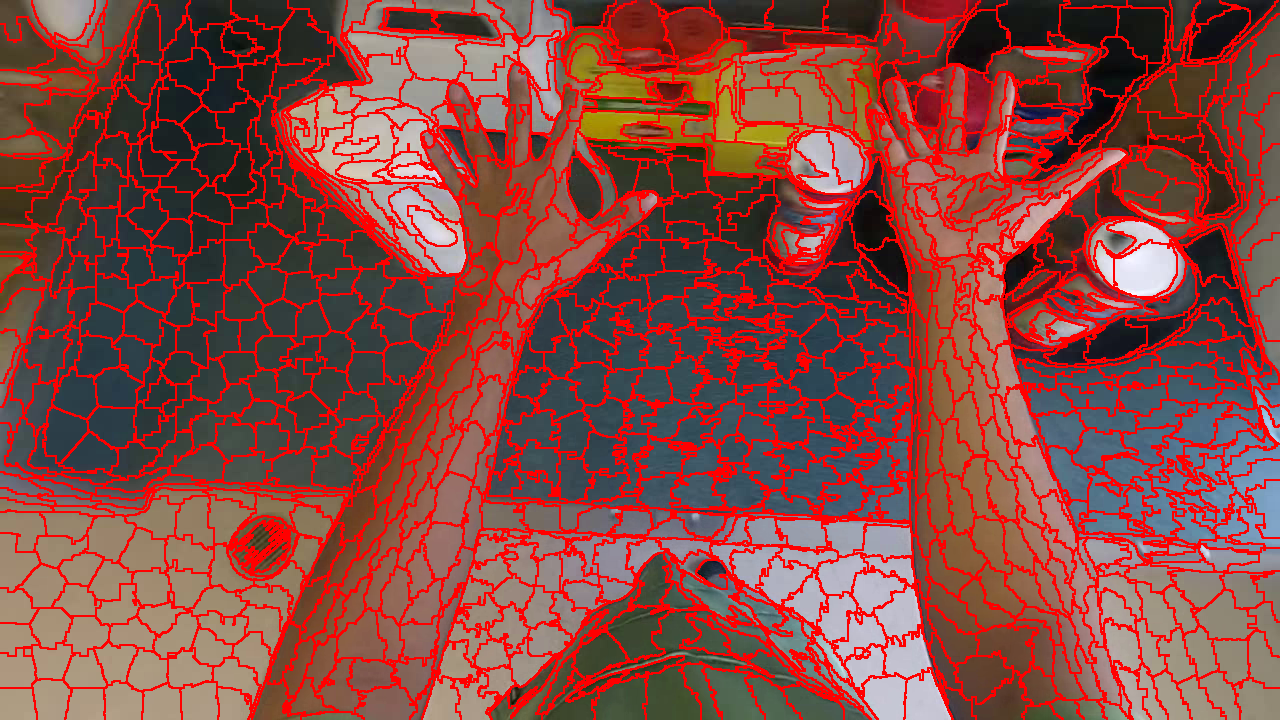
\includegraphics[width=\textwidth]{resources/images/m_basso_5.png}
		\caption{$m = 5$, $N = 1~000$}\label{es_bad_superpixel_m_basso}
	\end{subfigure}%
	\hfill
	\begin{subfigure}[t]{.495\textwidth}
		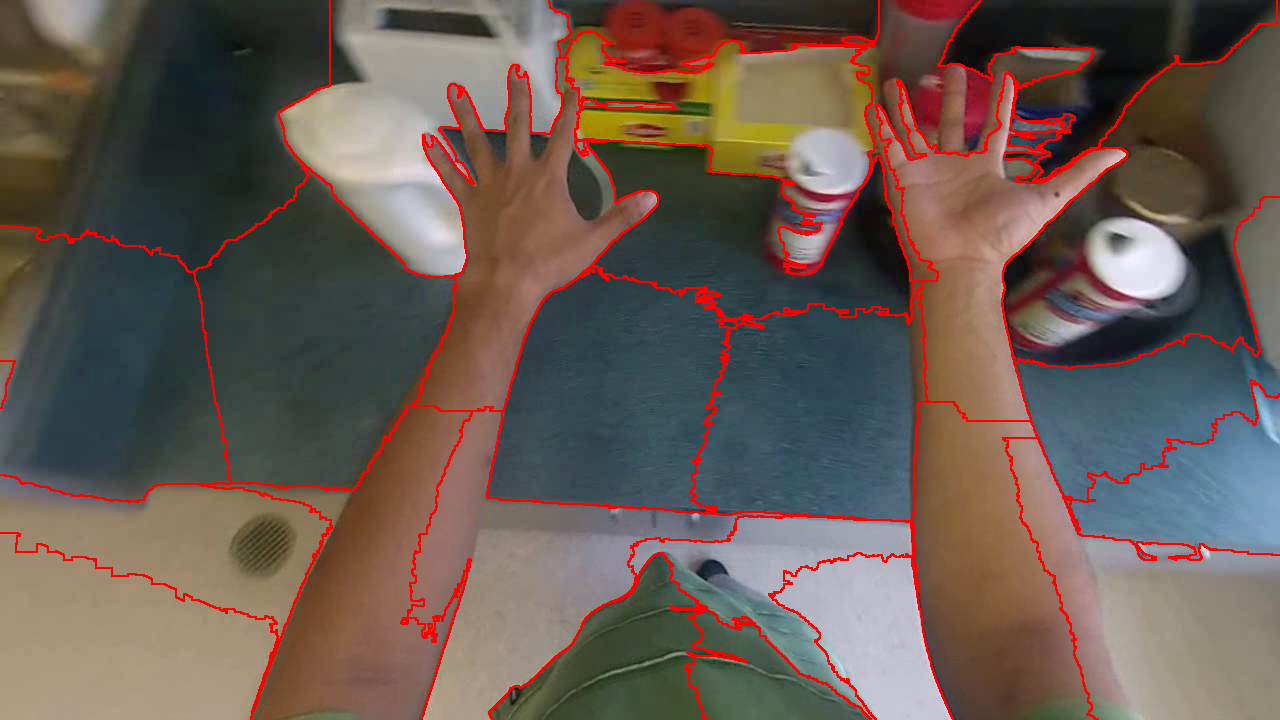
\includegraphics[width=\textwidth]{resources/images/N_basso_30.png}
		\caption{$N = 30$, $m = 30$}\label{es_bad_superpixel_N_basso}
	\end{subfigure}%
	\vspace{.0033\textwidth}
	\begin{subfigure}[t]{.495\textwidth}
		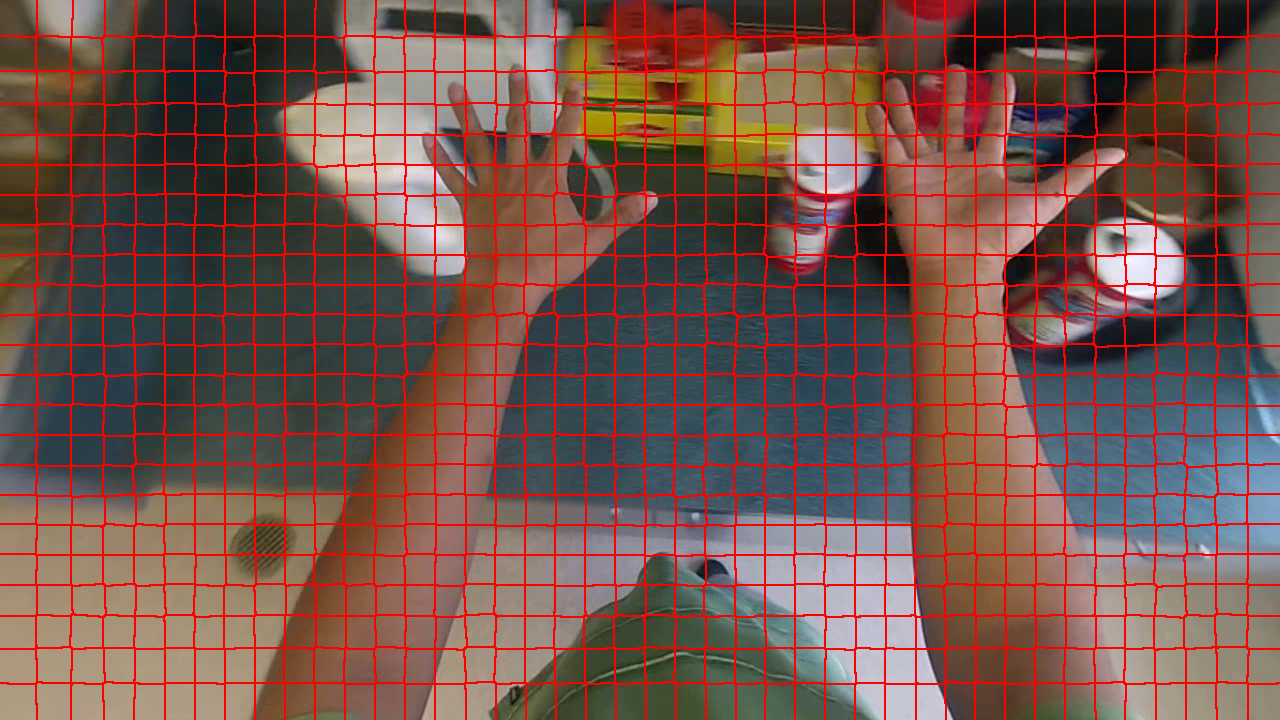
\includegraphics[width=\textwidth]{resources/images/m_alto_1000.png}
		\caption{$m = 1~000$, $N = 1~000$}\label{es_bad_superpixel_m_alto}
	\end{subfigure}%
	\hfill
	\begin{subfigure}[t]{.495\textwidth}
		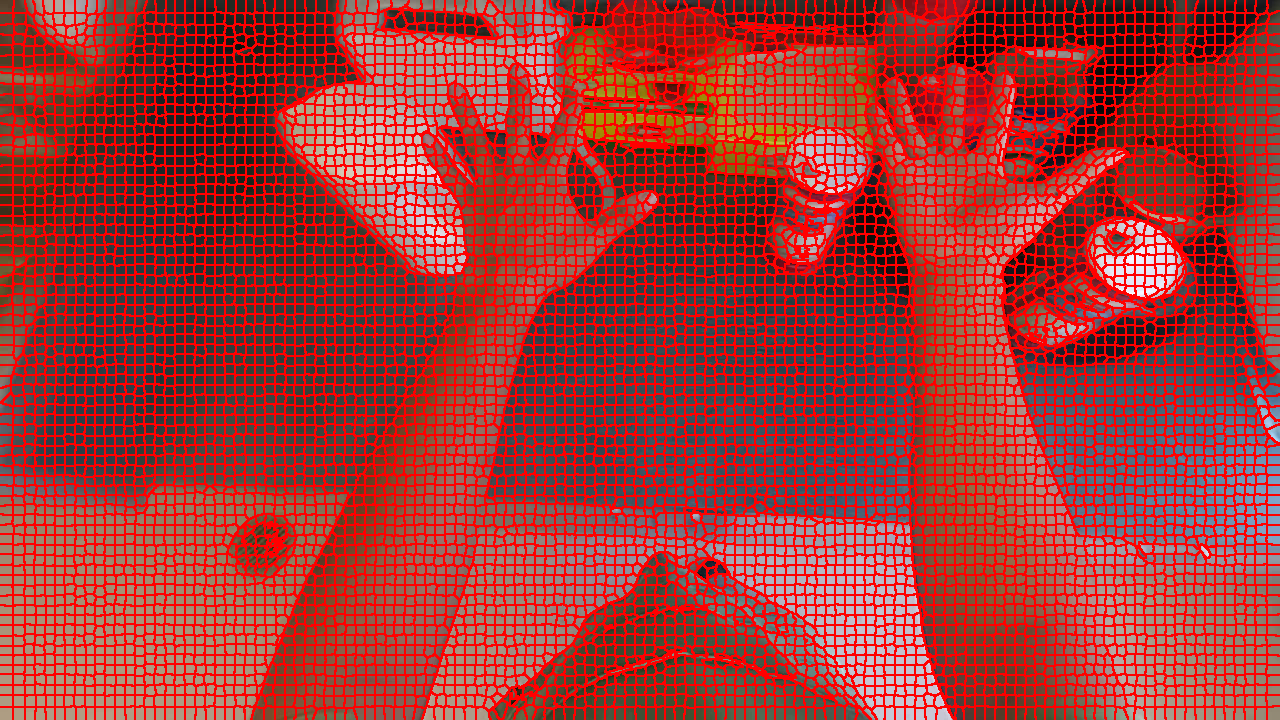
\includegraphics[width=\textwidth]{resources/images/N_alto_10000.png}
		\caption{$N = 10~000$, $m = 30$}\label{es_bad_superpixel_N_alto}
	\end{subfigure}%
	\caption{Esempio di errata suddivisione in superpixel}\label{es_bad_superpixel}
\end{figure}

\noindent La \cref{es_bad_superpixel} mostra alcuni esempi di errate suddivisioni in superpixel: nelle \cref{es_bad_superpixel_N_basso,es_bad_superpixel_m_basso} c'è poca uniformità nelle dimensioni dei superpixel, nella \cref{es_bad_superpixel_m_alto} non c'è aderenza ai bordi degli oggetti presenti nell'immagine mentre la \cref{es_bad_superpixel_N_alto} non è una rappresentazione di alto livello perché i \textit{cluster} sono piccoli quasi quanto i singoli pixel.

I dati mostrati nelle \cref{Iterazioni_vs_E_var_N,Iterazioni_vs_E_var_m} sono ottenuti mantenendo costante il numero di iterazioni, per poi misurare l'errore residuo medio $E$ calcolando la media dei singoli errori di ogni frame del video. In particolare, scegliendo gli stessi valori utilizzati nelle tabelle precedenti, ovvero un numero di iterazioni fisso a $10$, un fattore peso $m$ uguale a $30$ e un numero desiderato di superpixel $N$ pari a $1~000$, si può verificare che sussiste la relazione: $10~iterazioni \Leftrightarrow E \approx 0.37~px$.

Se invece di fissare inizialmente il numero di ripetizioni per poi ricavare $E$, si decide di procedere al contrario, ovvero si sceglie prima una soglia di errore massimo $E_{th}$ e dopo si misura il numero medio di iterazioni necessarie per raggiungere tale soglia, si ottengono risultati analoghi a quelli presentati nelle \cref{Iterazioni_vs_E_var_N,Iterazioni_vs_E_var_m}. Pertanto, mediamente, impostare una soglia di errore $E_{th}$ equivale a utilizzare un numero costante di iterazioni. Tuttavia, considerando i singoli frame invece del video nella sua interezza, fissare $E_{th}$ garantisce una maggiore precisione, dato che con un numero fisso di ripetizioni non si può avere la certezza che l'errore sia minore o uguale a $E_{th}$ per ogni fotogramma del filmato. È importante inoltre notare che il valore minimo di $E_{th}$ deve essere scelto con criterio: si è visto che per $N$ e $m$ piccoli è necessario un alto numero di iterazioni, fissando quindi una soglia di errore troppo bassa si rischia che il numero di ripetizioni necessarie per la convergenza sia eccessivamente grande o che la convergenza non venga raggiunta proprio.  

\begin{table}[!htb]
	\renewcommand{\arraystretch}{1.3}
	\centering
	\begin{tabular}{|c||>{\centering\arraybackslash}m{.26\textwidth}|>{\centering\arraybackslash}m{.21\textwidth}|>{\centering\arraybackslash}m{.17\textwidth}|}
	    \hline
		\multirow{2}{*}{\vspace{-6ex}Video}
		& \multicolumn{3}{c|}{VideoSLIC}\\\cline{2-4}
		& Tempo di esecuzione medio per frame [ms] & Scarto quadratico medio $\sigma$ [ms] & Numero medio di iterazioni\\
		\hline\hline
		\texttt{EDSH1.avi} & $304.2$ & $27.22$ & $17.6$ \\\hline
		\texttt{EDSH2.avi} & $304.1$ & $25.88$ & $17.6$ \\\hline
		\texttt{EDSHK.avi} & $295.6$ & $19.25$ & $17.2$ \\\hline\hline
		Media              & $301.3$ & $24.12$ & $17.5$ \\\hline
	\end{tabular}
	\caption{Prestazioni imponendo una soglia di errore pari a $0.25~px$}
	\label{EDSH_videos_error_no_memory}
\end{table}
\noindent In questa tesi si decide di impostare $E_{th} = 0.25~px$. Ciò significa imporre la condizione che in media i superpixel possano modificare la loro posizione (ovvero il loro centro) di un quarto di pixel al massimo fra iterazioni consecutive. Un superpixel può cambiare la sua posizione media solamente in due modi: acquisendo e/o cedendo singoli pixel da e verso altri superpixel. La soglia di errore viene dunque raggiunta quando i pixel scambiati fra \textit{cluster} diversi sono in quantità tale da rendere lo spostamento medio dei centri dei superpixel minore o uguale a $E_{th}$. La \cref{EDSH_videos_error_no_memory} mostra i risultati ottenuti fissando $E_{th} = 0.25~px$, $m = 30$ e $N = 1~000$.

\subsubsection{Elaborazione dei frame con memoria ed effetto \textit{drifting}}\label{Drifting_effect}
Considerando un filmato come un flusso di immagini interconnesse fra loro, è lecito pensare che le informazioni ottenute per i superpixel di un certo frame si possano trasmettere anche al frame successivo. Si ipotizza dunque che, per quanto debole, ci sia un qualche legame di correlazione tra due frame consecutivi. La \cref{EDSH_videos_error_memory} mostra i risultati che si ottengono sfruttando questo legame: la suddivisione in superpixel e i relativi centri di ogni \textit{cluster} ricavati da un determinato fotogramma vengono utilizzati, senza subire alcuna modifica, per inizializzare anche il frame seguente, pertanto tali informazioni rappresentano la ``memoria'' dell'elaborazione.
\begin{table}[!htb]
	\renewcommand{\arraystretch}{1.3}
	\centering
	\begin{tabular}{|c||>{\centering\arraybackslash}m{.26\textwidth}|>{\centering\arraybackslash}m{.21\textwidth}|>{\centering\arraybackslash}m{.17\textwidth}|}
	    \hline
		\multirow{2}{*}{\vspace{-6ex}Video}
		& \multicolumn{3}{c|}{VideoSLIC}\\\cline{2-4}
		& Tempo di esecuzione medio per frame [ms] & Scarto quadratico medio $\sigma$ [ms] & Numero medio di iterazioni\\
		\hline\hline
		\texttt{EDSH1.avi} & $58.1$ & $23.96$ & $3.1$ \\\hline
		\texttt{EDSH2.avi} & $70.0$ & $30.22$ & $3.9$ \\\hline
		\texttt{EDSHK.avi} & $84.3$ & $40.72$ & $4.9$ \\\hline\hline
		Media              & $71.6$ & $31.88$ & $4.0$ \\\hline
	\end{tabular}
	\captionsetup{justification=centering}
	\caption{Prestazioni con memoria imponendo $E_{th} = 0.25~px$, $m = 30$ e $N = 1~000$}
	\label{EDSH_videos_error_memory}
\end{table}
\\Le prestazioni ottenute sfruttando l'interconnessione dei frame (\cref{EDSH_videos_error_memory}) sono nettamente migliori rispetto a quelle dove ogni fotogramma viene processato indipendentemente dagli altri (\cref{EDSH_videos_error_no_memory}), tuttavia la qualità della segmentazione in superpixel diminuisce proporzionalmente alla durata del video considerato a causa dell'effetto \textit{drifting}, rendendo questo approccio utilizzabile nella pratica solo per filmati molto brevi (nell'ordine di alcuni secondi).
\begin{figure}[!htb]
	\centering
	\begin{subfigure}[t]{.49\textwidth}
		\begin{tikzpicture}[x=.16\textwidth,y=-.16\textwidth]
			\draw[step=.16\textwidth,gray,very thin,line cap=rect] (0,0) grid (5,4);
			\node[above left] at (-.1,-.1) {\small$0$};
			\node[above] at (1,-.1) {\small$S$};
			\node[left] at (-.1,1) {\small$S$~};
			\foreach \x in {2,...,4} \node[above] at (\x,-.1) {\small\x$S$};
			\foreach \y in {2,...,3} \node[left] at (-.1,\y) {\small\y$S$};
			\foreach \x in {2.2} \foreach \y in {1.9} \foreach \z in {violet} \filldraw[dashed,thick,line cap=rect,color=\z,fill opacity=.5] (\x-1,\y-1) rectangle (\x+1,\y+1);
			\filldraw[dashed,thick,line cap=rect,color=brown,fill opacity=.5] (1.5,0.0) -- (1.5,1.8) -- (3.5,1.8) -- (3.5,0.0) -- cycle;
			\foreach \x in {2.8} \foreach \y in {1.7} \foreach \z in {blue} \filldraw[dashed,thick,line cap=rect,color=\z,fill opacity=.5] (\x-1,\y-1) rectangle (\x+1,\y+1);
			\foreach \x in {1.6} \foreach \y in {1.5} \foreach \z in {red} \filldraw[dashed,thick,line cap=rect,color=\z,fill opacity=.5] (\x-1,\y-1) rectangle (\x+1,\y+1);
			\draw[ultra thick,color=violet,<-] (2.2,3.4) -- (2.2,2.9);
			\draw[ultra thick,color=brown,<-] (2.5,-0.5) -- (2.5,0.0);
			\draw[ultra thick,color=blue,<-] (4.3,1.7) -- (3.8,1.7);
			\draw[ultra thick,color=red,<-] (0.1,1.5) -- (0.6,1.5);
			\draw[<->,ultra thick] (0,4) node (yaxis) [below] {$y$} |- (5,0) node (xaxis) [right] {$x$};
		\end{tikzpicture}
		\caption{Con l'avanzare del video, i centri dei superpixel (e le relative aree $2S \times 2S$ che li circondano) si allontanano progressivamente gli uni dagli altri}
	\end{subfigure}%
	\hfill
	\begin{subfigure}[t]{.49\textwidth}
		\begin{tikzpicture}[x=.16\textwidth,y=-.16\textwidth]
			\draw[step=.16\textwidth,gray,very thin,line cap=rect] (0,0) grid (5,4);
			\node[above left] at (-.1,-.1) {\small$0$};
			\node[above] at (1,-.1) {\small$S$};
			\node[left] at (-.1,1) {\small$S$~};
			\foreach \x in {2,...,4} \node[above] at (\x,-.1) {\small\x$S$};
			\foreach \y in {2,...,3} \node[left] at (-.1,\y) {\small\y$S$};
			\foreach \x in {2.2} \foreach \y in {2.7} \foreach \z in {violet} \filldraw[dashed,thick,line cap=rect,color=\z,fill opacity=.5] (\x-1,\y-1) rectangle (\x+1,\y+1);
			\filldraw[dashed,thick,line cap=rect,color=brown,fill opacity=.5] (1.5,0.0) -- (1.5,1.3) -- (3.5,1.3) -- (3.5,0.0) -- cycle;
			\foreach \x in {3.8} \foreach \y in {2.1} \foreach \z in {blue} \filldraw[dashed,thick,line cap=rect,color=\z,fill opacity=.5] (\x-1,\y-1) rectangle (\x+1,\y+1);
			\foreach \x in {1.3} \foreach \y in {1.3} \foreach \z in {red} \filldraw[dashed,thick,line cap=rect,color=\z,fill opacity=.5] (\x-1,\y-1) rectangle (\x+1,\y+1);
			\fill[color=green,opacity=.5] (2.3,1.3) rectangle (2.8,1.7);
			\draw[<->,ultra thick] (0,4) node (yaxis) [below] {$y$} |- (5,0) node (xaxis) [right] {$x$};
		\end{tikzpicture}
		\caption{La zona verde non è più raggiungibile perché troppo distante dai centri dei superpixel adiacenti}
	\end{subfigure}%
	\hfill
	\begin{subfigure}[t]{.49\textwidth}
		\begin{tikzpicture}[x=.16\textwidth,y=-.16\textwidth]
			\draw[step=.16\textwidth,gray,very thin,line cap=rect] (0,0) grid (5,4);
			\node[above left] at (-.1,-.1) {\small$0$};
			\node[above] at (1,-.1) {\small$S$};
			\node[left] at (-.1,1) {\small$S$~};
			\foreach \x in {2,...,4} \node[above] at (\x,-.1) {\small\x$S$};
			\foreach \y in {2,...,3} \node[left] at (-.1,\y) {\small\y$S$};
			\filldraw[color=violet,fill opacity=.5] (1.4,2.3) -- (2.3,1.7) -- (2.8,1.7) -- (3.0,2.0) -- (3.2,2.9) -- (2.8,3.5) -- (1.7,3.3) -- cycle;
			\filldraw[color=brown,fill opacity=.5] (2.0,0.1) -- (1.7,0.5) -- (2.3,1.3) -- (2.8,1.3) -- (3.5,1.1) -- (3.3,0.2) -- cycle;
			\filldraw[color=red,fill opacity=.5] (0.6,0.9) -- (1.7,0.5) -- (2.3,1.3) -- (2.3,1.7) -- (1.4,2.3) -- (0.8,2.3) -- cycle;
			\filldraw[color=blue,fill opacity=.5] (2.8,1.3) -- (3.5,1.1) -- (4.2,1.4) -- (4.1,2.7) -- (3.2,2.9) -- (3.0,2.0) -- (2.8,1.7) -- (2.3,1.7) -- (2.3,1.3)-- cycle;
			\draw[<->,ultra thick] (0,4) node (yaxis) [below] {$y$} |- (5,0) node (xaxis) [right] {$x$};
		\end{tikzpicture}
	\end{subfigure}%
	\hfill
	\begin{subfigure}[t]{\textwidth}
		\caption{La regione non raggiungibile rimane comunque assegnata al superpixel a cui apparteneva in precedenza (in questo esempio il \textit{cluster} di colore blu). Il superpixel blu presenta dunque un margine sinistro di forma rettangolare che però non rispecchia i contorni dell'immagine e indica quindi la comparsa dell'effetto \textit{drifting}}
	\end{subfigure}
\caption{Spiegazione grafica dell'effetto \textit{drifting}}\label{es_drifting_explanation}
\end{figure}
\\L'effetto \textit{drifting} (illustrato graficamente nella \cref{es_drifting_explanation}) è una conseguenza dell'elaborazione dei frame con memoria e consiste nella comparsa di superpixel con alcuni bordi rettilinei che ricordano forme triangolari e/o rettangolari. Viene chiamato \textit{drifting} perché è il risultato dell'allontanamento progressivo dei centri dei \textit{cluster} gli uni dagli altri. È dovuto al fatto che l'algoritmo \gls{SLIC} esegue una ricerca locale in un'area $2S \times 2S$ per ogni centro e quindi, se i centri dei superpixel sono troppo distanti fra loro, alcune regioni dell'immagine non sono raggiungibili dalla ricerca. Ogni volta che si processa un nuovo frame, queste regioni rimangono attribuite allo stesso \textit{cluster} di appartenenza del fotogramma precedente, e restano tali fino a quando non possono essere riassegnate a un nuovo superpixel sufficientemente vicino in termini di spazio. I contorni regolari assunti dai superpixel a causa dell'effetto \textit{drifting} sono una conseguenza del fatto che l'area di ricerca locale $2S \times 2S$ è un quadrato e quindi le zone non raggiungibili dalla ricerca sono delimitate da quadrati o da loro intersezioni.
\begin{figure}[!htb]	
	\centering
	\begin{subfigure}[t]{.325\textwidth}
		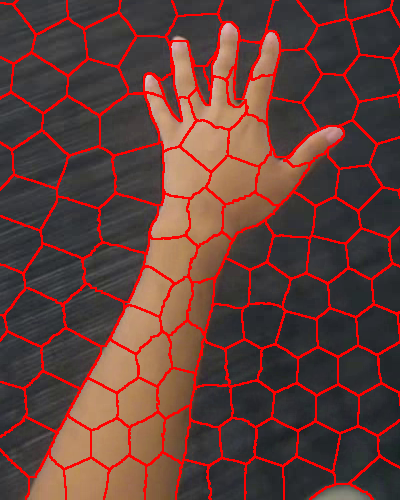
\includegraphics[width=\textwidth]{resources/images/drifting300a.png}
		\captionsetup{justification=centering}
		\caption{Segmentazione lievemente errata (contorni)}\label{es_drifting_300a}
	\end{subfigure}%
	\hfill
	\begin{subfigure}[t]{.325\textwidth}
		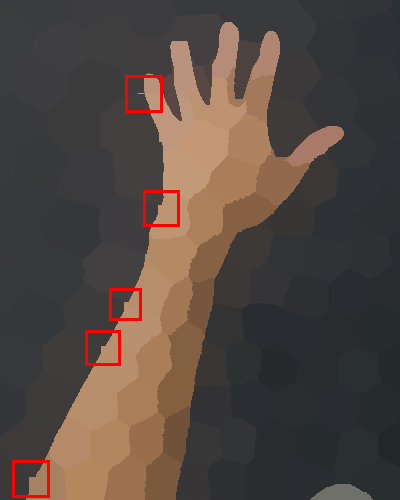
\includegraphics[width=\textwidth]{resources/images/drifting300b.png}
		\captionsetup{justification=centering}
		\caption{Segmentazione lievemente errata\\(colore medio)}\label{es_drifting_300b}
	\end{subfigure}%
	\hfill
	\begin{subfigure}[t]{.325\textwidth}
		
\includegraphics[width=\textwidth]{resources/images/drifting300c.png}
		\captionsetup{justification=centering}
		\caption{Segmentazione corretta}
	\end{subfigure}%
	\vspace{.0033\textwidth}
	\begin{subfigure}[t]{.325\textwidth}
		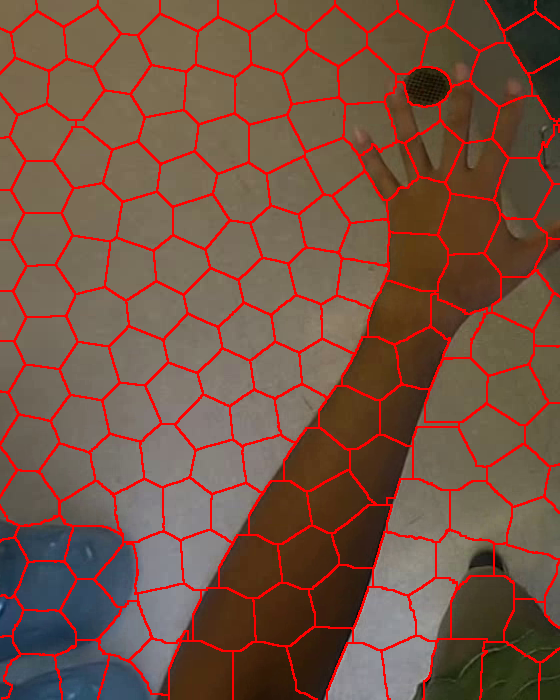
\includegraphics[width=\textwidth]{resources/images/drifting1100a.png}
		\captionsetup{justification=centering}
		\caption{Segmentazione palesemente errata (contorni)}\label{es_drifting_1100a}
	\end{subfigure}%
	\hfill
	\begin{subfigure}[t]{.325\textwidth}
		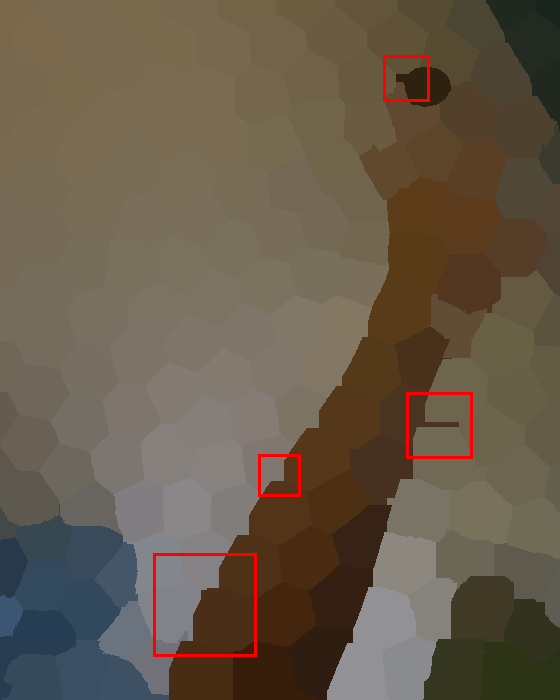
\includegraphics[width=\textwidth]{resources/images/drifting1100b.png}
		\captionsetup{justification=centering}
		\caption{Segmentazione palesemente errata\\(colore medio)}\label{es_drifting_1100b}
	\end{subfigure}%
	\hfill
	\begin{subfigure}[t]{.325\textwidth}
		
\includegraphics[width=\textwidth]{resources/images/drifting1100c.png}
		\captionsetup{justification=centering}
		\caption{Segmentazione corretta}
	\end{subfigure}%
	\caption{Esempio di effetto \textit{drifting}}\label{es_drifting}
\end{figure}
\\Le \cref{es_drifting_300a,es_drifting_300b} mostrano l'influenza dell'effetto \textit{drifting} sulla segmentazione in superpixel del video \texttt{EDSH1.avi} dopo l'elaborazione di circa $300$ frame, mentre le \cref{es_drifting_1100a,es_drifting_1100b} illustrano le conseguenze dopo aver processato un migliaio di fotogrammi. Più si avanza nel filmato, più l'effetto \textit{drifting} interferisce impedendo una corretta suddivisione in superpixel.

\subsubsection{Utilizzo di frame chiave e filtraggio bayesiano}\label{Risultati_filtraggio}
L'effetto \textit{drifting} compare solamente quando si elaborano i frame con memoria, ovvero tenendo conto dei legami che intercorrono tra fotogrammi consecutivi, pertanto è sufficiente non considerare tali legami se si vogliono evitare effetti indesiderati. Tuttavia, utilizzare l'approccio con memoria comporta una notevole riduzione dei tempi di esecuzione del programma, perciò in questa tesi vengono proposte due possibili soluzioni per limitare l'impatto dell'effetto \textit{drifting} senza dover rinunciare al miglioramento delle prestazioni: l'uso di frame chiave e l'impiego del filtraggio bayesiano.

Il primo metodo è il più semplice e si basa sull'azzeramento frequente della memoria di elaborazione, attuabile mediante l'inizializzazione a default di fotogrammi a intervalli regolari. La scelta della lunghezza di tali intervalli dipende da quanto si è disposti a tollerare l'effetto \textit{drifting}: più gli intervalli sono estesi, più tale effetto risulta evidente, anche se le prestazioni ne traggono vantaggio. Una buona regola empirica consiste tuttavia nell'impostare la cadenza dei frame chiave in funzione del \textit{frame rate} del video considerato. I filmati dell'\textit{EDSH dataset}~\cite{KITANI_HAND_DETECTION} sono girati a $30~fps$, pertanto si decide di fissare la frequenza dei frame chiave a $1/30$. In altri termini, la memoria di elaborazione viene reimpostata dopo ogni secondo trascorso di video. I risultati ottenuti sono mostrati nella \cref{EDSH_videos_key_frames} (con $E_{th} = 0.25~px$, $m = 30$ e $N = 1~000$).
\begin{table}[!htb]
	\renewcommand{\arraystretch}{1.29}
	\centering
	\begin{tabular}{|c||>{\centering\arraybackslash}m{.26\textwidth}|>{\centering\arraybackslash}m{.21\textwidth}|>{\centering\arraybackslash}m{.17\textwidth}|}
	    \hline
		\multirow{2}{*}{\vspace{-6ex}Video}
		& \multicolumn{3}{c|}{VideoSLIC}\\\cline{2-4}
		& Tempo di esecuzione medio per frame [ms] & Scarto quadratico medio $\sigma$ [ms] & Numero medio di iterazioni\\
		\hline\hline
		\texttt{EDSH1.avi} & $193.7$ & $56.27$ & $            10.9$ \\\hline
		\texttt{EDSH2.avi} & $196.2$ & $57.98$ & $            11.1$ \\\hline
		\texttt{EDSHK.avi} & $177.4$ & $74.66$ & $\hspace{.5em}9.9$ \\\hline\hline
		Media              & $189.1$ & $62.97$ & $            10.6$ \\\hline
	\end{tabular}
	\caption{Prestazioni con memoria ricorrendo ai frame chiave}
	\label{EDSH_videos_key_frames}
\end{table}

\noindent La seconda soluzione al problema dell'effetto \textit{drifting} è meno immediata, si ispira al filtro di Kalman e consiste nell'aggiunta di rumore gaussiano alla posizione dei centri dei superpixel. Non riuscendo infatti a modellare con precisione la complessa dinamica dei video presi in esame, si ritiene che una buona approssimazione sia tuttavia data dal considerare la posizione attuale dei centri dei \textit{cluster} uguale a quella del frame precedente, con l'aggiunta di una certa quantità di rumore gaussiano. Variare verso l'alto l'intensità di tale rumore comporta un peggioramento delle prestazioni perché sono necessarie più iterazioni per la convergenza dell'errore (dato che la posizione dei centri cambia molto da fotogramma a fotogramma), mentre una variazione verso il basso corrisponde a tempi di esecuzione più contenuti, fino al caso limite in cui il rumore è nullo e quindi si hanno gli stessi risultati già presentati nella \cref{EDSH_videos_error_memory}. Considerando le proprietà della funzione densità di probabilità gaussiana e il passo di campionamento $S$ dell'algoritmo, è buona norma scegliere $\sigma$ in modo da avere $3\sigma \leq S$, che equivale a garantire uno spostamento dei centri dei superpixel minore di $S$ in più del $99~\%$ dei casi (infatti è alquanto improbabile che un \textit{cluster} modifichi più di così la sua posizione media da un frame al successivo). La \cref{EDSH_videos_noise} illustra i risultati ottenuti impostando $\sigma = S/5$ (con $E_{th} = 0.25~px$, $m = 30$ e $N = 1~000$).
\begin{table}[!htb]
	\renewcommand{\arraystretch}{1.3}
	\centering
	\begin{tabular}{|c||>{\centering\arraybackslash}m{.26\textwidth}|>{\centering\arraybackslash}m{.21\textwidth}|>{\centering\arraybackslash}m{.17\textwidth}|}
	    \hline
		\multirow{2}{*}{\vspace{-6ex}Video}
		& \multicolumn{3}{c|}{VideoSLIC}\\\cline{2-4}
		& Tempo di esecuzione medio per frame [ms] & Scarto quadratico medio $\sigma$ [ms] & Numero medio di iterazioni\\
		\hline\hline
		\texttt{EDSH1.avi} & $165.8$ & $34.52$ & $            10.0$ \\\hline
		\texttt{EDSH2.avi} & $156.3$ & $29.14$ & $\hspace{.5em}9.5$ \\\hline
		\texttt{EDSHK.avi} & $147.3$ & $38.12$ & $\hspace{.5em}9.0$ \\\hline\hline
		Media              & $156.5$ & $33.93$ & $\hspace{.5em}9.5$ \\\hline
	\end{tabular}
	\caption{Prestazioni con memoria e aggiunta di rumore gaussiano}
	\label{EDSH_videos_noise}
\end{table}

\noindent È interessante notare che nelle \cref{EDSH_videos_key_frames,EDSH_videos_noise} i dati sono ricavati senza impostare alcun vincolo sul numero di iterazioni, eppure si ottiene un numero medio di ripetizioni molto prossimo a $10$, che è lo stesso consigliato dagli autori di \cite{ACHANTA_SLIC}. Questo fatto conferma la bontà del criterio di convergenza adottato dagli ideatori di \gls{SLIC}~\cite{ACHANTA_SLIC}.

Combinando le due soluzioni proposte (utilizzo di frame chiave insieme a filtraggio bayesiano) si hanno le prestazioni mostrate nella \cref{EDSH_videos_key_frames_noise} (i parametri utilizzati sono gli stessi delle \cref{EDSH_videos_key_frames,EDSH_videos_noise}).

\begin{table}[!htb]
	\renewcommand{\arraystretch}{1.3}
	\centering
	\begin{tabular}{|c||>{\centering\arraybackslash}m{.26\textwidth}|>{\centering\arraybackslash}m{.21\textwidth}|>{\centering\arraybackslash}m{.17\textwidth}|}
	    \hline
		\multirow{2}{*}{\vspace{-6ex}Video}
		& \multicolumn{3}{c|}{VideoSLIC}\\\cline{2-4}
		& Tempo di esecuzione medio per frame [ms] & Scarto quadratico medio $\sigma$ [ms] & Numero medio di iterazioni\\
		\hline\hline
		\texttt{EDSH1.avi} & $241.2$ & $39.27$ & $13.5$ \\\hline
		\texttt{EDSH2.avi} & $243.3$ & $38.01$ & $13.7$ \\\hline
		\texttt{EDSHK.avi} & $224.4$ & $48.19$ & $12.6$ \\\hline\hline
		Media              & $236.3$ & $41.82$ & $13.3$ \\\hline
	\end{tabular}
	\captionsetup{justification=centering}
	\caption{Prestazioni con memoria, frame chiave e aggiunta di rumore gaussiano}
	\label{EDSH_videos_key_frames_noise}
\end{table}

\noindent Dal punto di vista qualitativo, la segmentazione in superpixel risulta migliore nel caso in cui si ricorra all'utilizzo di frame chiave: l'effetto \textit{drifting} diventa trascurabile poiché si presenta raramente e solo in zone circoscritte del fotogramma. Applicando invece il modello bayesiano che coinvolge l'impiego di rumore gaussiano, l'effetto \textit{drifting} continua a manifestarsi, ma in maniera abbastanza limitata e tollerabile se si è disposti a scendere a compromessi sulla qualità dei superpixel per favorire le prestazioni. Combinare le due soluzioni aumenta i tempi di esecuzione senza però comportare benefici significativi in termini qualitativi.

La \cref{EDSH_videos_conclusion} mostra una sintesi dei principali punti di forza e degli svantaggi più evidenti che caratterizzano le varie implementazioni dell'algoritmo viste finora.

\begingroup
\renewcommand{\arraystretch}{1.3}
\begin{longtable}[!htb]{|>{\centering\arraybackslash}m{.2\textwidth}||>{\centering\arraybackslash}m{.14\textwidth}|>{\raggedright\arraybackslash}m{.25\textwidth}|>{\raggedright\arraybackslash}m{.25\textwidth}|}

	\multicolumn{4}{r}{\footnotesize\tablename~\thetable: continua nella pagina seguente}\\
	\endfoot
	\endlastfoot
	
	\hline
	Tipo di elaborazione video & Dati di riferimento & \multicolumn{1}{>{\raggedright\arraybackslash}c|}{Vantaggi} & \multicolumn{1}{>{\raggedright\arraybackslash}c|}{Svantaggi}\\
	\hline\hline
	Senza memoria, con numero fisso di iterazioni & \Cref{EDSH_videos_perf_mthread} &
	{\textcolor{blue}{$+$}} discrete prestazioni
	\newline{\textcolor{blue}{$+$}} effetto \textit{drifting} assente &
	{\textcolor{red}{$-$}} livello di errore non controllabile\\\hline
	Senza memoria, con soglia di errore           & \Cref{EDSH_videos_error_no_memory} & {\textcolor{blue}{$+$}} livello di errore controllabile
	\newline{\textcolor{blue}{$+$}} effetto \textit{drifting} assente &
	{\textcolor{red}{$-$}} prestazioni migliorabili\\\hline
	Con memoria e soglia di errore               & \Cref{EDSH_videos_error_memory} & 
	{\textcolor{blue}{$+$}} livello di errore controllabile
	\newline{\textcolor{blue}{$+$}} ottime prestazioni &
	{\textcolor{red}{$-$}} effetto \textit{drifting} accentuato, che rende questo metodo di fatto inutilizzabile\\\hline
	Con memoria, soglia di errore e frame chiave & \Cref{EDSH_videos_key_frames} & {\textcolor{blue}{$+$}} livello di errore controllabile
	\newline{\textcolor{blue}{$+$}} discrete prestazioni
	\newline{\textcolor{blue}{$+$}} effetto \textit{drifting} trascurabile &
	{\textcolor{red}{$-$}} nessuno\\\hline
	Con memoria, soglia di errore e aggiunta rumore       & \Cref{EDSH_videos_noise} & {\textcolor{blue}{$+$}} livello di errore controllabile
	\newline{\textcolor{blue}{$+$}} discrete prestazioni &
	{\textcolor{red}{$-$}} effetto \textit{drifting}, anche se limitato
	\newline{\textcolor{red}{$-$}} necessari calcoli supplementari\\\hline
	Con memoria, soglia di errore, frame chiave e aggiunta rumore       & \Cref{EDSH_videos_key_frames_noise} & {\textcolor{blue}{$+$}} livello di errore controllabile
	\newline{\textcolor{blue}{$+$}} effetto \textit{drifting} trascurabile &
	{\textcolor{red}{$-$}} prestazioni migliorabili
	\newline{\textcolor{red}{$-$}} necessari calcoli supplementari\\\hline
	
	\captionsetup{justification=centering}
	\caption{Riepilogo di vantaggi e svantaggi delle implementazioni di VideoSLIC}
	\label{EDSH_videos_conclusion}
\end{longtable}
\endgroup

\subsection{Connettività dei superpixel}
L'algoritmo trattato finora non garantisce esplicitamente la connettività dei superpixel, ovvero non è assicurato che tutti i pixel appartenenti a un determinato \textit{cluster} siano contigui: potrebbero infatti verificarsi situazioni in cui alcuni punti di un certo superpixel siano ``isolati'' dal resto del \textit{cluster} (la \cref{connectivity_graph} chiarisce meglio questo concetto). Generalmente il problema della connettività si presenta quando vengono elaborate immagini con zone molto irregolari, come possono essere l'erba di un prato oppure un terreno ricoperto di pietrisco. In questi casi l'algoritmo ha difficoltà a creare superpixel uniformi, e quindi produce come risultato \textit{cluster} molto frammentati. Per ovviare a tale inconveniente è necessario implementare una procedura ricorsiva da aggiungere all'algoritmo, la quale allunga però inevitabilmente i tempi di esecuzione del programma, pertanto occorre valutare con attenzione l'importanza di garantire o meno la connettività.
\begin{figure}[!htb]
	\centering
	\begin{subfigure}[t]{.49\textwidth}
		\begin{tikzpicture}[x=.16\textwidth,y=-.16\textwidth]
			\draw[step=.16\textwidth,gray,very thin,line cap=rect] (0,0) grid (5,4);
			\node[above left] at (-.1,-.1) {\small$0$};
			\node[above] at (1,-.1) {\small$S$};
			\node[left] at (-.1,1) {\small$S$~};
			\foreach \x in {2,...,4} \node[above] at (\x,-.1) {\small\x$S$};
			\foreach \y in {2,...,3} \node[left] at (-.1,\y) {\small\y$S$};
			\foreach \x in {2.2} \foreach \y in {2.3} \foreach \z in {violet} \filldraw[dashed,thick,line cap=rect,color=\z,fill opacity=.5] (\x-1,\y-1) rectangle (\x+1,\y+1);
			\filldraw[dashed,thick,line cap=rect,color=brown,fill opacity=.5] (1.5,0.0) -- (1.5,1.3) -- (3.5,1.3) -- (3.5,0.0) -- cycle;
			\foreach \x in {3.2} \foreach \y in {2.1} \foreach \z in {blue} \filldraw[dashed,thick,line cap=rect,color=\z,fill opacity=.5] (\x-1,\y-1) rectangle (\x+1,\y+1);
			\foreach \x in {1.6} \foreach \y in {1.3} \foreach \z in {red} \filldraw[dashed,thick,line cap=rect,color=\z,fill opacity=.5] (\x-1,\y-1) rectangle (\x+1,\y+1);
			\draw[<->,ultra thick] (0,4) node (yaxis) [below] {$y$} |- (5,0) node (xaxis) [right] {$x$};
		\end{tikzpicture}
		\caption{Area di ricerca di ogni superpixel}
	\end{subfigure}%
	\hfill
	\begin{subfigure}[t]{.49\textwidth}
		\begin{tikzpicture}[x=.16\textwidth,y=-.16\textwidth]
			\draw[step=.16\textwidth,gray,very thin,line cap=rect] (0,0) grid (5,4);
			\node[above left] at (-.1,-.1) {\small$0$};
			\node[above] at (1,-.1) {\small$S$};
			\node[left] at (-.1,1) {\small$S$~};
			\foreach \x in {2,...,4} \node[above] at (\x,-.1) {\small\x$S$};
			\foreach \y in {2,...,3} \node[left] at (-.1,\y) {\small\y$S$};
			\filldraw[color=brown,fill opacity=.5] (2.0,0.1) -- (1.7,0.5) -- (2.4,1.3) -- (3.5,1.1) -- (3.3,0.2) -- cycle;
			\filldraw[even odd rule,color=red,fill opacity=.5] (0.9,0.9) -- (1.7,0.5) -- (2.4,1.3) -- (2.3,1.7) -- (1.6,2.3) -- (0.9,2.0) -- cycle
			(1.95,1.6) circle (.15);
			\filldraw[even odd rule,color=blue,fill opacity=.5] (3.5,1.1) -- (3.8,1.4) -- (3.7,2.4) -- (3.0,2.5) -- (2.3,1.7) -- (2.4,1.3) -- cycle
			(2.75,1.8) circle (.15);
			\filldraw[color=violet,fill opacity=.5] (1.6,2.3) -- (2.3,1.7) -- (3.0,2.5) -- (2.6,3.0) -- (1.7,2.8) -- cycle
			(1.95,1.6) circle (.15)
			(2.75,1.8) circle (.15);
			\draw[<->,ultra thick] (0,4) node (yaxis) [below] {$y$} |- (5,0) node (xaxis) [right] {$x$};
		\end{tikzpicture}
		\caption{Il superpixel di colore viola ha due insiemi isolati di pixel che non sono contigui con il resto del \textit{cluster}}
	\end{subfigure}%
\caption{Illustrazione grafica di superpixel non connessi}\label{connectivity_graph}
\end{figure}

\noindent In questa tesi, la connettività dei superpixel si ritiene utile nel caso di elaborazione di singole immagini, ma non indispensabile quando si trattano filmati: i legami che intercorrono tra frame consecutivi contribuiscono in una certa misura a limitare la comparsa di \textit{cluster} frammentati. È importante inoltre notare che anche i \textit{cluster} frammentati contengono informazioni relative all'immagine elaborata, pertanto forzare la connettività di tali \textit{cluster} può equivalere a una perdita di dettagli della segmentazione.
\begin{table}[!htb]
	\renewcommand{\arraystretch}{1.26}
	\centering
	\begin{tabular}{|c||>{\centering\arraybackslash}m{.26\textwidth}|>{\centering\arraybackslash}m{.21\textwidth}|>{\centering\arraybackslash}m{.17\textwidth}|}
	    \hline
		\multirow{2}{*}{\vspace{-6ex}Video}
		& \multicolumn{3}{c|}{VideoSLIC}\\\cline{2-4}
		& Tempo di esecuzione medio per frame [ms] & Scarto quadratico medio $\sigma$ [ms] & Numero medio di iterazioni\\
		\hline\hline
		\texttt{EDSH1.avi} & $223.4$ & $53.18$ & $            10.2$ \\\hline
		\texttt{EDSH2.avi} & $225.4$ & $53.03$ & $            10.4$ \\\hline
		\texttt{EDSHK.avi} & $213.6$ & $68.73$ & $\hspace{.5em}9.6$ \\\hline\hline
		Media              & $220.8$ & $58.31$ & $            10.1$ \\\hline
	\end{tabular}
	\captionsetup{justification=centering}
	\caption{Prestazioni con memoria ricorrendo ai frame chiave e garantendo la connettività dei superpixel}
	\label{EDSH_videos_key_frames_connectivity}
\end{table}
\\La \cref{EDSH_videos_key_frames_connectivity} mostra le prestazioni che si ottengono garantendo la connettività dei \textit{cluster} (utilizzando gli stessi parametri della \cref{EDSH_videos_key_frames}): in particolare, si può notare come ciò comporti una leggera diminuzione delle iterazioni medie necessarie per la convergenza dell'errore, a fronte di un aumento dei tempi di esecuzione. Nella \cref{es_connectivity} si possono invece vedere le differenze che ci sono fra i superpixel non connessi e quelli connessi in un esempio concreto. 
\begin{figure}[!htb]	
	\centering
	\begin{subfigure}[t]{.495\textwidth}
		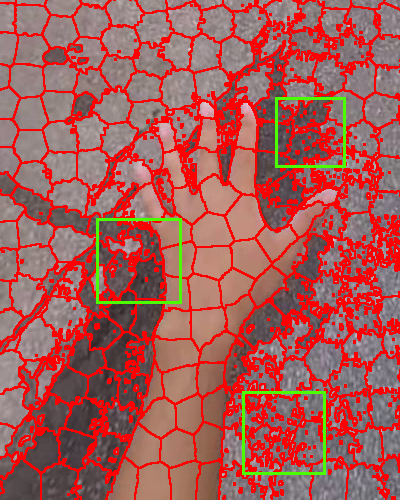
\includegraphics[width=\textwidth]{resources/images/connectivity_no.png}
		\caption{Superpixel non connessi}
	\end{subfigure}%
	\hfill
	\begin{subfigure}[t]{.495\textwidth}
		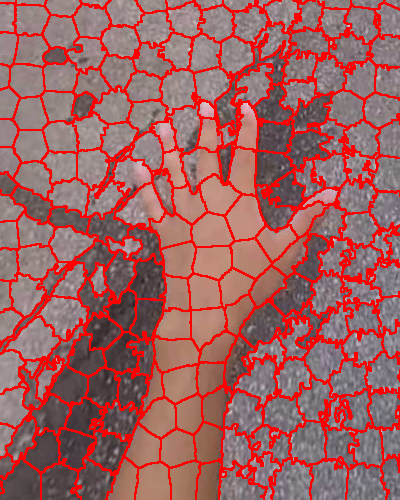
\includegraphics[width=\textwidth]{resources/images/connectivity_yes.png}
		\caption{Superpixel connessi}
	\end{subfigure}%
	\caption{Esempio di connettività dei superpixel}\label{es_connectivity}
\end{figure}

\subsection{Considerazioni sui tempi di esecuzione}
Tracciando i risultati ottenuti nelle \cref{EDSH_videos_perf_mthread,EDSH_videos_error_no_memory,EDSH_videos_error_memory,EDSH_videos_key_frames,EDSH_videos_noise,EDSH_videos_key_frames_noise} su un grafico (visibile in \cref{Iterazioni_vs_tempo}), si può osservare che il numero medio di iterazioni e il tempo medio di esecuzione per ogni fotogramma sono all'incirca direttamente proporzionali. Da tale relazione si può quindi dedurre che, per ottenere prestazioni prossime al tempo reale, è necessario avere un numero medio di ripetizioni minore di $2$. Questa considerazione vale ovviamente solo nel contesto specifico di svolgimento della tesi, ovvero tenendo conto del sistema hardware/software utilizzato e della risoluzione/\textit{frame rate} dei video dell'\textit{EDSH dataset}~\cite{KITANI_HAND_DETECTION}.
\begin{figure}[!htb]
\centering
\begin{tikzpicture}[scale=.9]
	\begin{axis}[
	    width=\textwidth,
		height=.7\textwidth,
		clip marker paths=true,
		grid=major,
		xmin=0,
		xmax=19,
		ymin=0,
		ymax=335,
		xtick={0,2,...,18},
		ytick={50,100,...,300},
		legend cell align=left,
		xlabel=\textit{Numero medio di iterazioni},
		ylabel={\textit{Tempo medio di esecuzione} [\textit{ms}]},
		tick pos=left,
		legend pos=north west,
		every axis legend/.append style={nodes={text depth=,text width=.3\textwidth}}
		]
		\addplot[no marks,dashed,red] coordinates {
		(1.0,25.29)
		(4.0,71.6)
		};		
		\addplot[mark=square*,mark size=.2em,red] coordinates {
		(4.0,71.6)
		(9.5,156.5)
		(10.0,178.5)
		(10.6,189.1)
		(13.3,236.3)
		(17.5,301.3)
		};
		\addplot[black,dashed,thick] coordinates {
		(0,33.33)
		(19,33.33)
		};
		\legend{,,soglia prestazioni \textit{real time} a $30~fps$};
	\end{axis}
\end{tikzpicture}
\captionsetup{justification=centering}
\caption{Relazione fra numero di iterazioni e tempo di esecuzione (per frame)}\label{Iterazioni_vs_tempo}
\end{figure}

\noindent La \cref{es_real_time} illustra la mediocre qualità della segmentazione in superpixel che si deve accettare se si vogliono ottenere prestazioni in tempo reale (il numero di iterazioni viene fissato a $1$).

\begin{figure}[!htb]	
	\centering
	\begin{subfigure}[t]{.495\textwidth}
		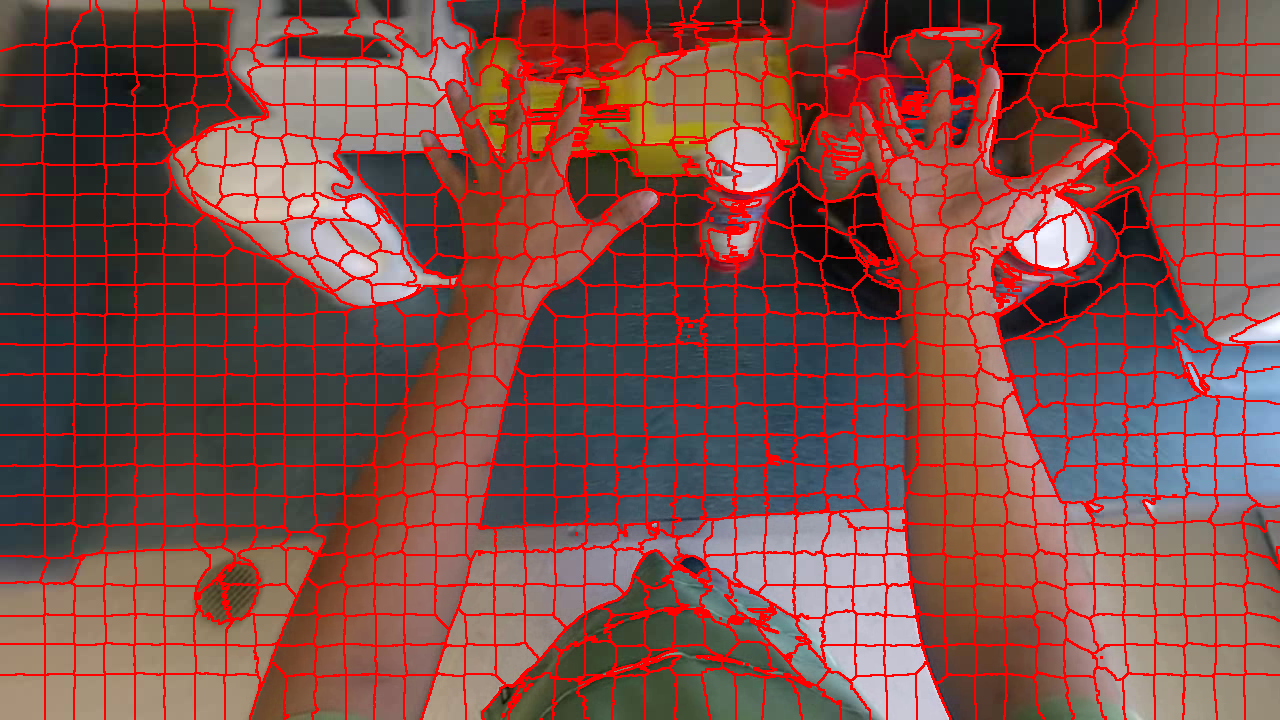
\includegraphics[width=\textwidth]{resources/images/realtime_contorni.png}
		\caption{Contorni dei \textit{cluster}}
	\end{subfigure}%
	\hfill
	\begin{subfigure}[t]{.495\textwidth}
		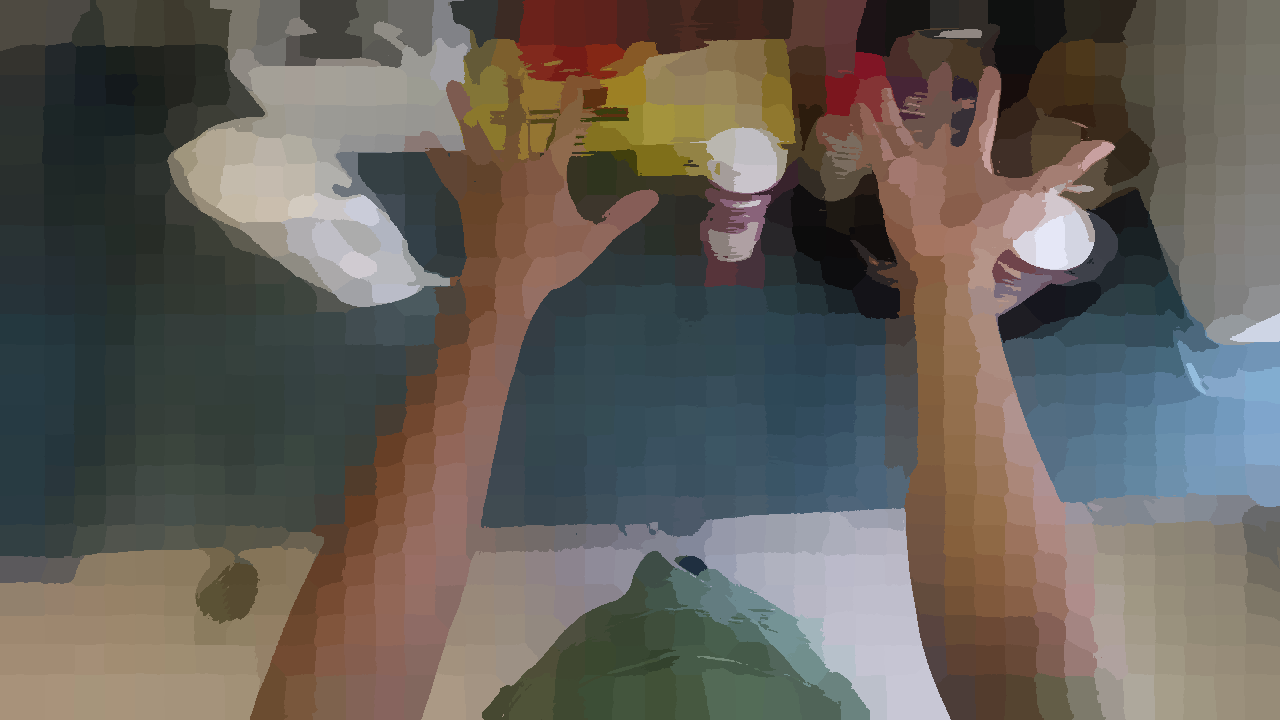
\includegraphics[width=\textwidth]{resources/images/realtime_superpixel.png}
		\caption{Colore medio dei \textit{cluster}}
	\end{subfigure}%
	\caption{Qualità dei superpixel con prestazioni in tempo reale}\label{es_real_time}
\end{figure}

\noindent Un ulteriore modo per abbreviare i tempi di esecuzione (nell'ordine di qualche millisecondo), senza peggiorare di molto la qualità dei \textit{cluster}, consiste nel modificare il metodo con cui viene calcolata la distanza nel colore. Ricordando che le immagini elaborate dall'algoritmo \gls{SLIC} vengono prima convertite allo spazio colore \mbox{LAB} (come in \cref{es_LAB}), si può scegliere di considerare solo il canale L (\cref{es_LAB_L}) al fine di calcolare la distanza. Tale canale contiene infatti le informazioni relative alla luminosità dell'immagine, costituendo dunque una rappresentazione in scala di grigi della stessa che ne risalta i contorni, mentre gli altri due canali A (\cref{es_LAB_A}) e B (\cref{es_LAB_B}) contengono informazioni sul colore. Il problema di questo approccio è la scarsa qualità dei superpixel nelle zone dell'immagine dove la luminosità resta pressoché costante mentre varia solo il colore, pertanto in questo elaborato di laurea si decide di includere tutti e tre i canali \mbox{LAB} nel calcolo della distanza.
\begin{figure}[!htb]	
	\centering
	\begin{subfigure}[t]{.495\textwidth}
		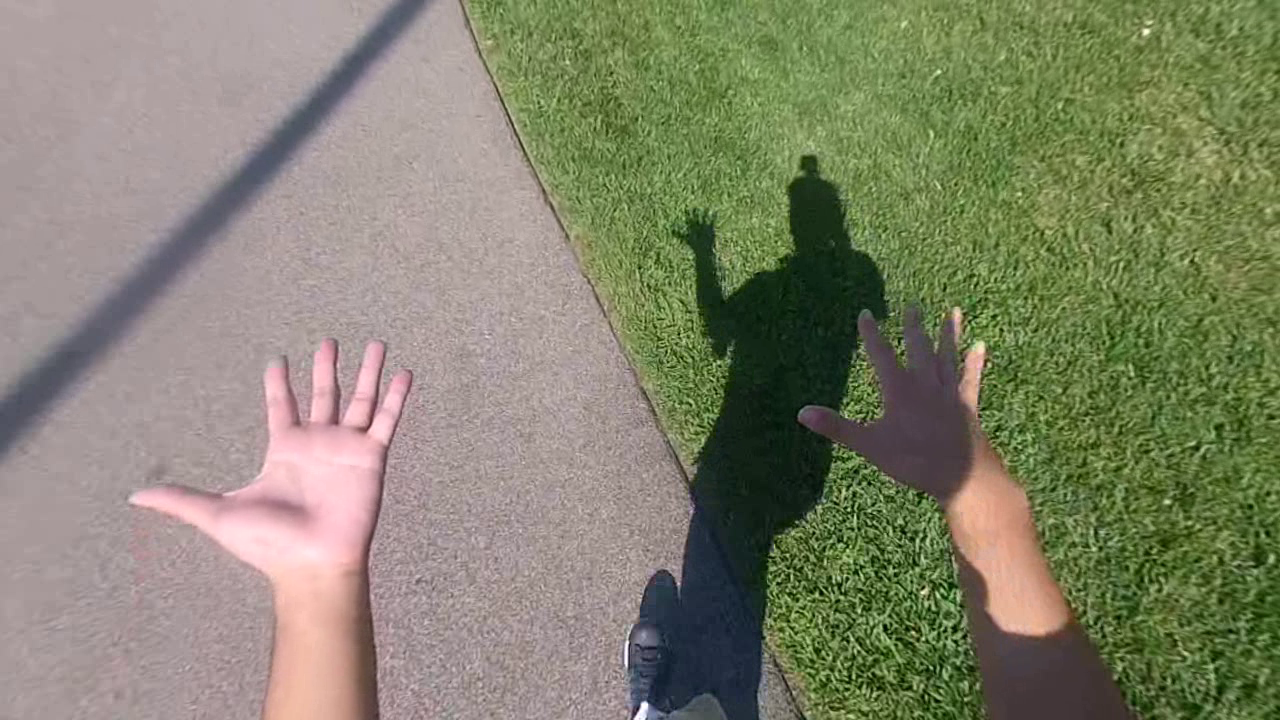
\includegraphics[width=\textwidth]{resources/images/es_LAB.png}
		\caption{Immagine originale}
	\end{subfigure}%
	\hfill
	\begin{subfigure}[t]{.495\textwidth}
		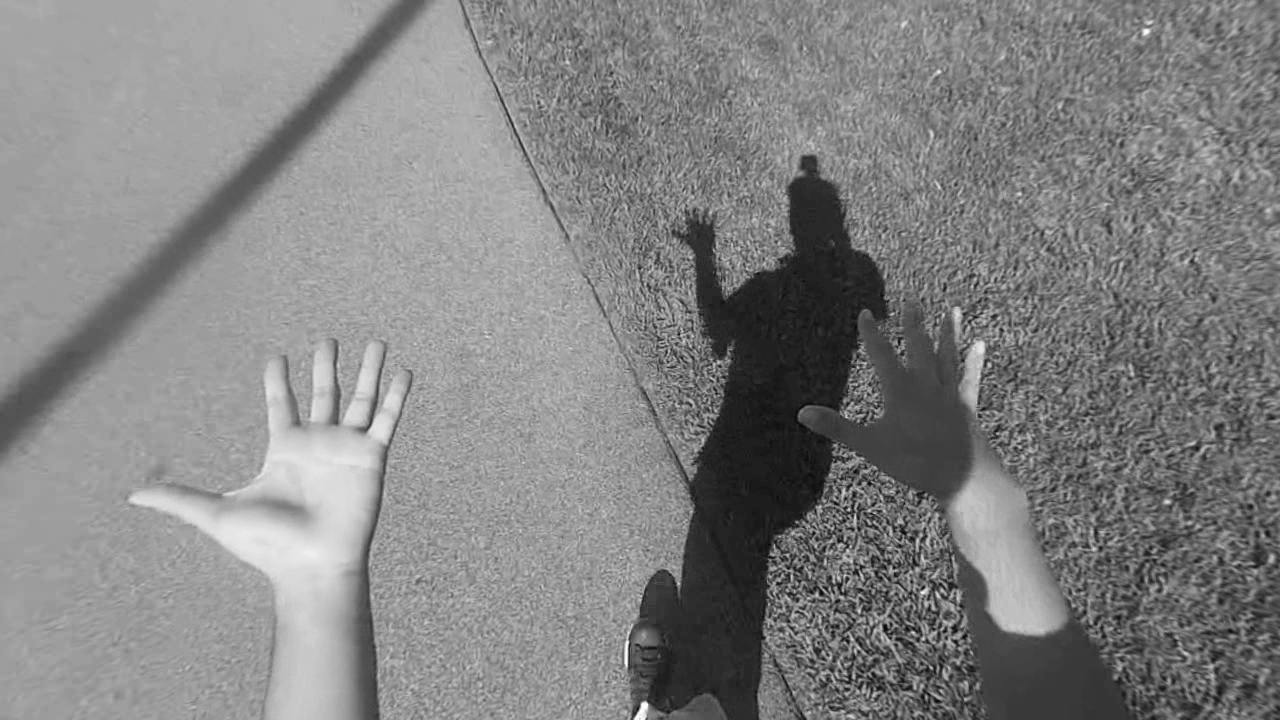
\includegraphics[width=\textwidth]{resources/images/es_LAB_L.png}
		\caption{Canale L dello spazio \mbox{LAB}}\label{es_LAB_L}
	\end{subfigure}%
	\vspace{.0033\textwidth}
	\begin{subfigure}[t]{.495\textwidth}
		
\includegraphics[width=\textwidth]{resources/images/es_LAB_A.png}
		\caption{Canale A dello spazio \mbox{LAB}}\label{es_LAB_A}
	\end{subfigure}%
	\hfill
	\begin{subfigure}[t]{.495\textwidth}
		
\includegraphics[width=\textwidth]{resources/images/es_LAB_B.png}
		\caption{Canale B dello spazio \mbox{LAB}}\label{es_LAB_B}
	\end{subfigure}%
	\caption{Esempio di immagine nello spazio colore \mbox{LAB}}\label{es_LAB}
\end{figure}
\newpage





\section{Conclusioni e Sviluppi Futuri}\label{Conclusioni}


In questa tesi si è scelto un algoritmo \cite{ACHANTA_SLIC} per la generazione di superpixel a partire da immagini e, con alcune modifiche, lo si è adattato affinché sia utilizzabile per applicazioni in ambito video. Si è visto che per avere buone prestazioni non è sufficiente elaborare i frame di un filmato indipendentemente gli uni dagli altri, ma bisogna considerare la correlazione tra fotogrammi consecutivi.
Sfruttando il legame che c'è tra un frame e quello successivo si è riusciti a ottenere ottimi tempi di esecuzione, a svantaggio però della qualità della segmentazione in superpixel, compromessa a causa dell'effetto \textit{drifting}. Volendo dunque mantenere alte sia le prestazioni sia la qualità dei \textit{cluster} si è dovuto ricorrere all'introduzione di frame chiave e a un modello probabilistico inspirato al filtraggio bayesiano.

L'obiettivo di adattare l'algoritmo \cite{ACHANTA_SLIC} alle sequenze video è stato raggiunto, poiché il programma sviluppato durante questo elaborato di laurea risulta pienamente funzionante. Per quanto riguarda invece il lavoro di ottimizzazione, è stato fatto il possibile per rendere il programma implementato operativo in tempo reale, ma con gli strumenti a disposizione e considerando i filmati dell'\textit{EDSH dataset}~\cite{KITANI_HAND_DETECTION} non si è riusciti a conseguire tale risultato mantenendo contemporaneamente una qualità accettabile della suddivisione in superpixel. Per video di risoluzioni e/o \textit{frame rate} sufficientemente bassi è possibile ottenere prestazioni in tempo reale, però il progresso tecnologico comporta filmati di dimensioni e qualità sempre maggiori, pertanto è necessario continuare il lavoro di ottimizzazione iniziato in questa tesi, tenendo presente che, in vista di un possibile impiego per le tecnologie indossabili, le risorse a disposizione sono limitate e per poterle sfruttare al massimo è necessario conoscere nel dettaglio il dispositivo che andrà a eseguire il programma. 

Come accennato nell'introduzione, il campo applicativo dei superpixel è vasto e i risultati finora ottenuti per le immagini possono essere estesi senza troppe difficoltà anche alle sequenze video. Riconoscimento, localizzazione e \textit{tracking} di oggetti all'interno delle scene dei filmati sono alcuni possibili esempi in cui la segmentazione in \textit{cluster} può risultare utile. Inoltre, con la diffusione di occhiali \textit{smart}, i superpixel potrebbero essere utilizzati per facilitare la realizzazione di applicazioni per la realtà aumentata. In tal senso, un altro possibile impiego non esaminato in questa tesi è il riconoscimento delle mani nei video girati in prima persona, similmente al lavoro svolto in \cite{SERRA_HAND_RECOGNITION}.

\noindent Questo elaborato di laurea lascia spazio a ulteriori approfondimenti e sviluppi futuri. Ad esempio, al posto di \gls{SLIC} si potrebbero applicare ai filmati altri algoritmi fra quelli citati, valutando e comparando i risultati per determinare il metodo migliore nella generazione di superpixel per le sequenze video. Inoltre, considerando un'elaborazione che tenga conto della correlazione tra frame, sarebbe interessante verificare se la comparsa dell'effetto \textit{drifting} dipende o meno dalla scelta dell'algoritmo da utilizzare, e nel caso tale effetto fosse comunque presente si potrebbe indagare più a fondo su approcci probabilistici più efficienti del modello ispirato al filtraggio bayesiano proposto nella tesi. Infine, si potrebbe cercare un metodo per ricavare i parametri necessari all'algoritmo \gls{SLIC} senza che ci sia bisogno di un intervento esterno, quindi in modo automatico direttamente dal filmato da elaborare (come ad esempio SLICO\footnote{SLIC \textit{zero parameter}: versione aggiornata di \gls{SLIC}, presentata sempre dagli autori di \cite{ACHANTA_SLIC}, che richiede come unico parametro il numero desiderato di superpixel}).





\newpage
\cleardoublepage
\phantomsection
\addcontentsline{toc}{section}{Bibliografia}
\bibliography{resources/bibliografia.bib}
\end{document}
